\documentclass[12pt,spanish,Letterpaper,openany]{book}
\usepackage{lmodern}
\usepackage{setspace}
\setstretch{0.85}
\usepackage{amssymb,amsmath}
\usepackage{ifxetex,ifluatex}
\usepackage{fixltx2e} % provides \textsubscript
\ifnum 0\ifxetex 1\fi\ifluatex 1\fi=0 % if pdftex
  \usepackage[T1]{fontenc}
  \usepackage[utf8]{inputenc}
\else % if luatex or xelatex
  \ifxetex
    \usepackage{mathspec}
  \else
    \usepackage{fontspec}
  \fi
  \defaultfontfeatures{Ligatures=TeX,Scale=MatchLowercase}
    \setmainfont[Scale=1.0, HyphenChar=None]{Corbel}
    \setsansfont[]{Corbel}
    \setmonofont[Mapping=tex-ansi]{Corbel}
\fi

\makeatletter
\renewcommand\mainmatter{\clearpage\@mainmattertrue\pagenumbering{arabic}}
\renewcommand\frontmatter{\clearpage\@mainmatterfalse\pagenumbering{arabic}}
\renewcommand\backmatter{\clearpage\@mainmatterfalse}
\makeatother

%\usepackage{etoolbox}
%\makeatletter
%\patchcmd{\@smemmain}{\cleardoublepage}{\clearpage}{}{}
%\patchcmd{\@smemmain}{\cleardoublepage}{\clearpage}{}{}
%\patchcmd{\@smemfront}{\cleardoublepage}{\clearpage}{}{}
%\patchcmd{\@smemfront}{\cleardoublepage}{\clearpage}{}{}
%\makeatother

\setlength{\parindent}{0em}

\usepackage{graphicx}
\usepackage{booktabs}
\usepackage{multicol}
\usepackage{doc}
\usepackage{float}
\usepackage{tcolorbox} 
\usepackage{lipsum}
\usepackage{tikz}
\usepackage{nonfloat}

\usepackage{pdfpages}

\usepackage[
contents={},
opacity=1,
scale=1.5,
color=blue!90
]{background}
\usepackage{lipsum}
\usepackage{ifthen}

\usepackage{xcolor}
\usepackage[pagestyles]{titlesec}

\renewpagestyle{plain}[\normalsize\sffamily\bfseries\slshape]{
  \setfoot{}{\color{black}{\thepage}}{}}

\newpagestyle{myps}[\normalsize\sffamily\bfseries\slshape]{
  \setfoot{}{\color{black}{\thepage}}{}}
  
\pagestyle{myps}


\usepackage{framed}
\definecolor{colorlinetitle}{HTML}{a87e00}%{a87e00}%
\definecolor{textlinetitle}{HTML}{061769}%{061769}%{061769}%
\definecolor{fondo}{HTML}{041d57}%
\definecolor{newfondo}{HTML}{3d0718}%
\colorlet{shadecolor}{fondo!81!}


% use upquote if available, for straight quotes in verbatim environments
\IfFileExists{upquote.sty}{\usepackage{upquote}}{}
% use microtype if available
\IfFileExists{microtype.sty}{%
\usepackage{microtype}
\UseMicrotypeSet[protrusion]{basicmath} % disable protrusion for tt fonts
}{}
\usepackage[inner=12.7mm,outer=12.7mm,top=23mm,bottom=18.5mm]{geometry}
\usepackage{hyperref}
\hypersetup{unicode=true,
            pdftitle={Revista digital de la escuela de ingeniería en Ciencias y Sistemas},
            pdfauthor={Escuela Ingenieria en Ciencias y Sistemas},
            pdfborder={0 0 0},
            breaklinks=true,
	  linkcolor=black,
	  urlcolor=gray}
\urlstyle{same}  % don't use monospace font for urls
\ifnum 0\ifxetex 1\fi\ifluatex 1\fi=0 % if pdftex
  \usepackage[shorthands=off,main=spanish]{babel}
\else
  \usepackage{polyglossia}
  \setmainlanguage[]{spanish}
\fi
\usepackage{natbib}
\bibliographystyle{apalike}
\usepackage{longtable,booktabs}
\IfFileExists{parskip.sty}{%
\usepackage{parskip}
}{% else
\setlength{\parindent}{0pt}
\setlength{\parskip}{6pt plus 2pt minus 1pt}
}
\setlength{\emergencystretch}{3em}  % prevent overfull lines
\providecommand{\tightlist}{%
  \setlength{\itemsep}{0pt}\setlength{\parskip}{0pt}}
\setcounter{secnumdepth}{5}
% Redefines (sub)paragraphs to behave more like sections
\ifx\paragraph\undefined\else
\let\oldparagraph\paragraph
\renewcommand{\paragraph}[1]{\oldparagraph{#1}\mbox{}}
\fi
\ifx\subparagraph\undefined\else
\let\oldsubparagraph\subparagraph
\renewcommand{\subparagraph}[1]{\oldsubparagraph{#1}\mbox{}}
\fi

%%% Use protect on footnotes to avoid problems with footnotes in titles
\let\rmarkdownfootnote\footnote%
\def\footnote{\protect\rmarkdownfootnote}


  \title{Revista digital de la escuela de ingeniería en Ciencias y Sistemas}
    \author{Escuela Ingenieria en Ciencias y Sistemas}
      \date{2024-10-15}

% no title page
\AtBeginDocument{\let\maketitle\relax}

\usepackage{caption2}
\captionsetup{%
labelsep=colon,%
font={footnotesize},%
aboveskip=0.4\baselineskip,%
belowskip=0\baselineskip,% deve essere 0 perché regolo lo spazio dal testo con \intextsep
}%

\usepackage{booktabs}
\usepackage{longtable}

\usepackage{indentfirst}
\setlength{\parindent}{1em}
\usepackage{enumitem}
\setlist[itemize]{labelindent = \parindent, leftmargin=*}

%\usepackage{framed,color}
%\definecolor{shadecolor}{RGB}{248,248,248}

\renewcommand{\textfraction}{0.05}
\renewcommand{\topfraction}{0.8}
\renewcommand{\bottomfraction}{0.8}
\renewcommand{\floatpagefraction}{0.75}

\renewcommand{\chaptername}{Artículo}
\addto\captionsspanish{\renewcommand{\chaptername}{Artículo}}
\addto\captionsspanish{\renewcommand{\contentsname}{Índice General}}


\frenchspacing
\tolerance=5000
\multicoltolerance=3000 

\raggedbottom
\raggedcolumns

\setlength{\columnsep}{1em}
%We want a rule between columns.
%\setlength\columnseprule{.4pt}

%Tambien queremos asegurarnos de que un nuevo entorno multicols 
%encuentre suficiente espacio en la parte inferior de la pagina.
\setlength\premulticols{6\baselineskip}

%Al equilibrar columnas, ignoramos las soluciones que son 
%demasiado malas. Ademas, si la ultima columna es demasiado mala, 
%la tipeamos sin estirar.
\setcounter{columnbadness}{7000}
\setcounter{finalcolumnbadness}{7000}

\newcommand{\prefacetitlecommand}%
{\titleformat{\chapter}[display]%
{\bfseries\large\color{colorlinetitle}}%
{\relax}%
{0ex}%
{{\titlerule[1.2pt]}\filright\color{textlinetitle}}[\color{colorlinetitle}\vspace{0.5ex}{\titlerule[1.2pt]}]%
}


\newcommand{\articletitlecommand}%
{\titleformat{\chapter}[display]%
{\bfseries\tiny\raggedright\color{white}}%
{\relax}%
{0ex}%
{}[\color{white}\vspace{0ex}{\titlerule[0pt]}]%
}



\newcommand{\sectionCenter}%
{\titleformat{\section}[block]%
{\bfseries\large\color{textlinetitle}\filcenter}%
{\relax}%
{0ex}%
{\empty}%
}


\newcommand{\sectionRight}%
{\titleformat{\section}[block]%
{\bfseries\large\color{textlinetitle}}%
{\relax}%
{0ex}%
{\empty}%
}


\newcommand{\subsectionRight}%
{\titleformat{\subsection}[block]%
{\bfseries\normalsize\color{textlinetitle}}%
{\relax}%
{0ex}%
{\empty}%
}

\usepackage{titletoc}
\titlecontents{chapter}[3em]
{\vspace{5mm}}
{\normalsize\contentslabel[\color{textlinetitle}\thecontentslabel]{2em}\color{black}\itshape\normalsize}
{\color{black}\itshape\normalsize}
{\color{colorlinetitle}\titlerule*[.3pc]{.}\color{black}\contentspage}

\newcommand{\tcolorboxcommand}{\begin{tcolorbox}[sharp corners=uphill, colback=newfondo, colframe=newfondo, arc=6mm, boxrule=0mm, boxsep=0mm]}

\newcommand{\photocommand}[2]{%
\fcolorbox[HTML]{DCEEA7}{DCEEA7}{%
\begin{minipage}{95.19mm}%
	\hspace{1mm}%
	\begin{minipage}{22.49mm}%
		\vspace{1mm}%
		\includegraphics[width=22.49mm, height=31.96mm]{#1}%
		\vspace{1mm}%
	\end{minipage}%
	\hspace{2.4mm}%
	\begin{minipage}{68.80mm}%
		#2
	\end{minipage}%
	\hspace{0.5mm}%
\end{minipage}%
}%
}

\definecolor{fondobiography}{HTML}{DCEEA7}

\NewDocumentEnvironment{photobiography}{m O{}}%
{%
\begin{tcolorbox}[colback=fondobiography, colframe=fondobiography, width=97.19mm, boxsep=-2mm, arc=0mm]
\begin{minipage}{95.19mm}%
	%\hspace{1mm}%
	\begin{minipage}{22.49mm}%
		\vspace{2mm}%
		\includegraphics[width=22.49mm, height=31.96mm]{#1}%
		\vspace{2mm}%
	\end{minipage}%
	\hspace{2.4mm}%
	\begin{minipage}{68.80mm}%
	#2%
}%
{%
	\end{minipage}%
	%\hspace{0.5mm}%
\end{minipage}%
\end{tcolorbox}
}


\newcommand{\spacetext}{\vspace{8.1mm}}
\newcommand{\minimalspacetext}{\vspace{1mm}}
\newcommand{\spaceelevenmilis}{\vspace{11mm}}
\newcommand{\spacetenmilis}{\vspace{10mm}}
\newcommand{\spaceninemilis}{\vspace{9mm}}
\newcommand{\spaceeightmilis}{\vspace{8mm}}
\newcommand{\spacesevenmilis}{\vspace{7mm}}
\newcommand{\spacesixmilis}{\vspace{6mm}}
\newcommand{\spacefivemilis}{\vspace{5mm}}
\newcommand{\spacefourmilis}{\vspace{4mm}}
\newcommand{\spacethreemilis}{\vspace{3mm}}
\newcommand{\spacetwomilis}{\vspace{2mm}}
\newcommand{\spaceinitialeditorialcontenido}{\vspace{8.1mm}}
\newcommand{\spaceoneminus}{\vspace{-1mm}}
\newcommand{\spacetwominus}{\vspace{-2mm}}
\newcommand{\spacefourminus}{\vspace{-4mm}}
\newcommand{\hideFromPandoc}[1]{#1}
\hideFromPandoc{ \let\Begin\begin \let\End\end }
\newcommand{\minipagepartone}{\begin{minipage}[c]{3cm}}
\newcommand{\minipagetwocolumn}{\noindent\begin{minipage}[c]{\columnwidth}}
\newcommand{\minipageparttwo}{\end{minipage}\begin{minipage}[c]{12cm}}
\newcommand{\minipageparttwochapter}{\end{minipage}\begin{minipage}[c]{15cm}}
\newcommand{\minipageendpart}{\end{minipage}}
\newcommand{\firstparteditorial}{\begin{longtable}[]{@{}ll@{}}\endhead\begin{minipage}[t]{0.47\columnwidth}\raggedright}
\newcommand{\firstparttwoeditorial}{\begin{longtable}[l]{@{}ll@{}}\endhead\begin{minipage}[t]{0.47\columnwidth}\raggedright}
\newcommand{\midleparteditorial}{\end{minipage} & \begin{minipage}[t]{0.47\columnwidth}\raggedright}
\newcommand{\lastparteditorial}{\end{minipage}\end{longtable}}

\newcommand{\HRule}{\begin{center}\rule{0.5\linewidth}{0.2mm}\end{center}}

\begin{document}
\maketitle

% \pagestyle{plain}

\includepdf{images/cover.pdf}

\AddEverypageHook{%
\ifthenelse{\value{page}<5}%
{\ifthenelse{\isodd{\value{page}}}%
  	{\backgroundsetup{scale=1, color=white, opacity=1, angle=0, contents={
\includegraphics[width=\paperwidth,height=\paperheight]{latex/background_numberimpar.pdf}}}}%
  	{\backgroundsetup{scale=1, color=white, opacity=1, angle=0, contents={
\includegraphics[width=\paperwidth,height=\paperheight]{latex/background_numberpar.pdf}}}}%
}{}%
\BgMaterial}

%%%%%%{
%%%%%%\setcounter{tocdepth}{0}
%%%\tableofcontents
%%%}
%%%%%%%%%%%%\listoffigures
%%%
\prefacetitlecommand

\titlespacing*{\chapter} {0pt}{0pt}{2pt}

\titleformat{\chapter}[display]
{\normalfont\color{black} \bfseries}
{\empty}
{0pt}
{\filcenter\Huge}

\spacetenmilis
\spacetenmilis
\spacetenmilis
\spacetenmilis

\begin{center}
\includegraphics[width=1\linewidth]{images/organigrama} \end{center}

\hypertarget{editorial}{%
\chapter*{Editorial}\label{editorial}}
\addcontentsline{toc}{chapter}{Editorial}

\begin{center}
\includegraphics[width=1\linewidth]{images/editorial} \end{center}

\setcounter{tocdepth}{0}
\tableofcontents

\articletitlecommand

\titlespacing*{\chapter} {0pt}{-60pt}{4pt}
%%%%%% SECCION 1 
\includepdf{images/seccion1.pdf}

\AddEverypageHook{%
\ifthenelse{\value{page}<17}%
{\ifthenelse{\isodd{\value{page}}}%
  	{\backgroundsetup{scale=1, color=white, opacity=1, angle=0, contents={
\includegraphics[width=\paperwidth,height=\paperheight]{latex/background_numberimpar.pdf}}}}%
  	{\backgroundsetup{scale=1, color=white, opacity=1, angle=0, contents={
\includegraphics[width=\paperwidth,height=\paperheight]{latex/background_numberpar.pdf}}}}%
}{}%
\BgMaterial}
%%%%%%%%%%%%%%%%%%%%%%%%%%%
\hypertarget{adrian}{%
\chapter{Del algoritmo a la acción: IA, Deep Learning y herramientas para impulsar el desarrollo tecnológico}\label{adrian}}

\begin{center}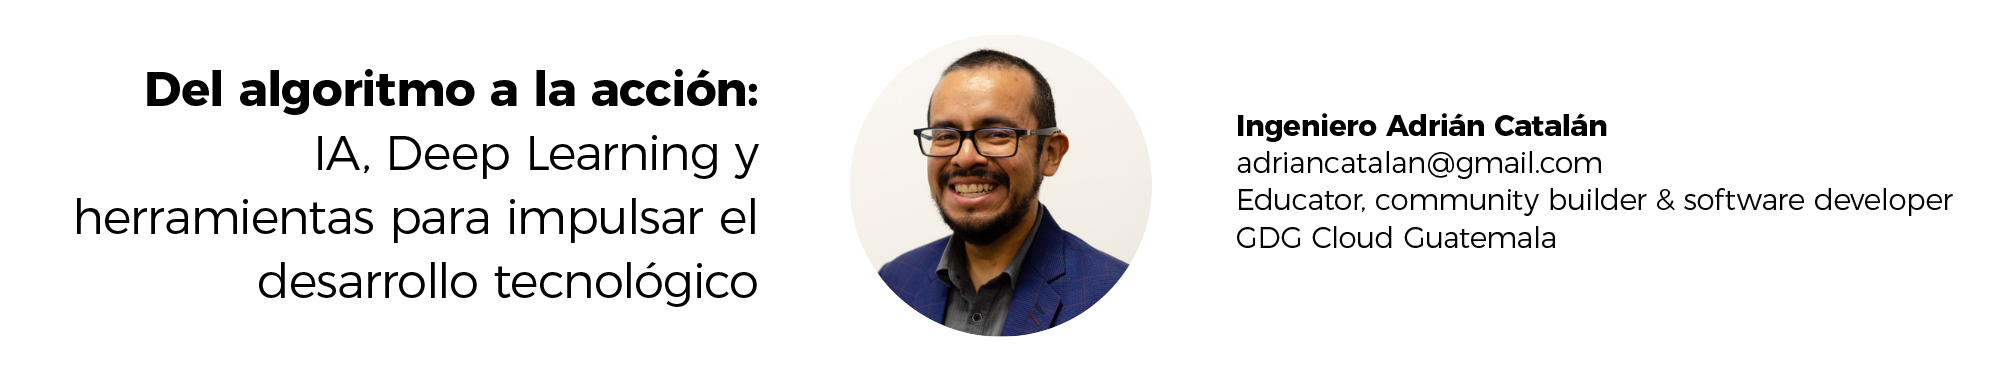
\includegraphics[width=1\linewidth]{autores/pareja00_adrian} \end{center}

\begin {multicols}{2}

\textbf{\emph{YouTube:}} \url{https://youtu.be/Uv4RSpL2jvE}

\hypertarget{entrevista}{%
\section{Entrevista}\label{entrevista}}

\textbf{¿Quién es Adrián Catalán?}

Soy un aprendiz eterno de la vida, siempre en busca de conocimiento. Dirijo el laboratorio de innovación en la Universidad Galileo desde hace más de 10 años, y también ofrezco consultorías en machine learning y desarrollo móvil. He organizado meetups y gracias a mi cercanía con Google, soy parte del programa de developer experts. Además de mis especialidades técnicas, tengo certificaciones en áreas no técnicas como sommelier, barista, bartender, y coach de vida, e incluso he explorado la comedia con stand up.

Esta diversidad de experiencias me ha proporcionado una perspectiva holística y humana. Sigo trabajando en tecnología y disfruto colaborar con personas. Recientemente, me apasiona el montañismo y el ultra maratón, lo que refleja mis intereses variados y el deseo de compartir mis habilidades tanto técnicas como personales.

\textbf{¿Cómo se involucró en la industria tecnológica?}

Estudié Ingeniería de Sistemas y he explorado diversas áreas en la industria tecnológica, evitando entornos muy burocráticos como los bancos, que no me interesan. He trabajado en seguridad informática, redes, desarrollo web, móvil y más recientemente en machine learning. Desde mis años universitarios, he estado involucrado en comunidades tecnológicas, como LUGUSAC y la Comunidad de Microsoft, y más tarde fundé el GDG, lo que me ha permitido conectar con muchos perfiles. Me apasiona compartir lo que aprendo y he sido conferencista en eventos nacionales e internacionales. Espero seguir involucrado con la comunidad por muchos años más.

\textbf{¿Qué son las comunidades tecnológicas y cómo pueden aportar al país?}

Las comunidades tecnológicas, o meetups, son espacios en Latinoamérica para reunir a personas con intereses similares en tecnología y compartir conocimientos, han crecido y adquirido su propia identidad. Por ejemplo, si me interesa Firebase, busco a otros que lo utilicen para colaborar, organizar eventos y proyectos. Estas comunidades son cruciales para el crecimiento del ecosistema de innovación y tecnología de un país, ofreciendo oportunidades de aprendizaje y networking, lo que impacta positivamente en el desarrollo económico y social. En resumen, se trata de reunir a personas con intereses comunes y fomentar la colaboración.

\textbf{¿Tecnologías en las que actualmente desarrolla sus proyectos?}

Tengo una buena relación con Google, aunque no soy empleado, solo me cubren los gastos de viaje, lo que permite acercarme a diferentes comunidades. Prefiero las tecnologías de Google, especialmente Google Cloud Platform (GCP), debido a su amplia oferta y su eficacia para acelerar prototipos y productos. He trabajado mucho con Firebase y tengo experiencia en Android, aunque también he explorado iOS.

Recientemente, me he enfocado en machine learning, usando herramientas como TensorFlow y Vertex. Creo que es crucial que la innovación técnica no solo sea efectiva, sino que también mejore la calidad de vida de las personas. Aunque me inclino por las tecnologías de Google, reconozco el valor de otras alternativas y estoy abierto a discutir diferentes implementaciones en mis consultorías.

\textbf{¿A qué se refiere con ``Del Algoritmo a la Acción''?}

Los algoritmos son fundamentales en cualquier producto tecnológico, y como ingenieros, trabajamos constantemente con ellos. Es crucial ir más allá de la teoría y enfocarse en implementar esos conceptos de manera práctica. El verdadero valor de un algoritmo radica en su aplicación y en el impacto positivo que puede tener en la vida de las personas, las empresas y la sociedad. Comenzamos con una idea teórica que se transforma en acción, dando lugar a soluciones concretas en productos tecnológicos que mejoran la calidad de vida.

\textbf{¿Qué es la IA para el Ing. Adrián Catalán?}

Me apasiona la inteligencia artificial, la veo como un concepto amplio que abarca el uso de tecnología para realizar tareas que antes se consideraban exclusivas de los humanos, con resultados igual o mejores. Detrás de esto hay diversos algoritmos, técnicas, hardware y software, siendo el machine learning y las redes neuronales algunas de las implementaciones más comunes.

Considero que la inteligencia artificial es una herramienta que complementa al ser humano, no lo reemplaza. Mejora la productividad y permite enfocarse en la innovación, optimizando recursos como dinero, esfuerzo y tiempo. Al dedicar menos a tareas repetitivas, podemos centrarnos en lo importante, lo que, al final, contribuye a una mejor calidad de vida.

\textbf{¿Cómo nace el concepto de Deep Learning?}

La inteligencia artificial (IA) como mencionaba es un concepto amplio, comparado a una sombrilla, bajo la cual se encuentra el aprendizaje automático (machine learning), que utiliza datos históricos para hacer predicciones a través de modelos. Dentro de machine learning, las redes neuronales, que simulan de manera básica el funcionamiento del cerebro humano, emplean operaciones matemáticas complejas para minimizar errores.

El deep learning, una subcategoría de machine learning, se caracteriza por tener múltiples capas (capas ocultas) que aumentan la profundidad del modelo. Aunque estas técnicas se exploraron en los años 80, no se pudieron desarrollar adecuadamente hasta alrededor de 2010, cuando se mejoraron gracias a la disponibilidad de más datos y poder computacional. Los avances actuales en IA se destacan en el procesamiento de lenguaje natural y la visión por computadora.

La IA se puede dividir en tres etapas: la específica (en la que estamos ahora), la general (a la que aspiramos) y la superior (más inteligente que el ser humano). Aunque se considera que la IA actual parece tener características de inteligencia general (como en modelos como chatGPT y Gemini), la realidad es que estamos en la etapa específica. En resumen, el deep learning utiliza redes neuronales para abordar problemas de machine learning, que a su vez son parte de la inteligencia artificial.

\textbf{¿En las etapas de desarrollo tecnológico de qué herramientas nos podemos apoyar?}

Soy un firme defensor de utilizar las herramientas disponibles en el momento, basándome en mis conocimientos, por muchos años di clases de estructuras de datos, compiladores y sistemas operativos; conocer las bases es clave para construir soluciones tecnológicas. No reinvento la rueda en cada proyecto; aprovecho plataformas colaborativas y la nube, como Firebase y Google Cloud, para escalar mis soluciones.

En el ámbito de inteligencia artificial, me gusta TensorFlow, aunque también existen opciones como PyTorch. Aunque inicialmente no me gustaba Python, aprendí a usarlo para IA, dado que otros lenguajes como Kotlin o Ruby tienen limitaciones en este campo. La comunidad también es crucial al elegir herramientas.

Recomiendo un stack que incluya TensorFlow y herramientas como Pandas y NumPy, montados en la infraestructura de la nube de Google, el uso Vertex para trabajar con APIs como Gemini. En resumen, se trata de conocer los fundamentos, utilizar lo que está disponible y resolver problemas de manera eficiente, buscando un producto final listo lo más rápido posible.

\textbf{Roles que pueden involucrarse durante las etapas de desarrollo como Machine Learning}

La respuesta sobre roles en machine learning es complicada debido a la tendencia y lo novedoso de la industria. Al igual que en la seguridad informática, donde los roles no siempre son claros, en machine learning a menudo se confunden las funciones de un científico de datos y un ingeniero de machine learning.

El científico de datos analiza datos para tomar decisiones, mientras que el ingeniero de machine learning se enfoca en automatizar estos procesos. En Guatemala, por ejemplo, es común ver equipos de ciencia de datos compuestos por ingenieros industriales y de sistemas.

Es esencial que cada persona entienda sus intereses y sepa comunicarlos a los empleadores. Así como en seguridad informática se ha integrado el concepto de DevSecOps, en machine learning se habla de MLOps, aunque su implementación varía entre empresas.

La limpieza de datos es crucial y a menudo complicada, por lo que contar con un ingeniero de datos es vital. En resumen, los roles se dividen así: el ingeniero de machine learning desarrolla modelos, el ingeniero de datos maneja y limpia los datos, y el científico de datos los analiza. Identificar intereses y buscar un buen ajuste con la empresa es clave para el éxito en este campo.

\textbf{¿Dónde es un buen comienzo para aprender? ¿Cómo iniciar, nos puede plantear escenarios?}

Como ingeniero de sistemas, creo que sería ideal tener más profesionales en este campo, aunque entiendo que ir a la universidad puede ser complicado en nuestro país. La universidad pública presenta desafíos de horarios y costos de oportunidad, y las privadas tienen sus propios costos.

Mi recomendación es optar por una institución educativa que ofrezca posgrados o cursos, o explorar plataformas en línea como Coursera, edX o Udemy. No todos aprendemos de la misma manera, así que es crucial encontrar el método que mejor se adapte a cada uno. Personalmente, me gusta aprender de forma práctica, como lo proponen cursos de Andrew Ng y Jeremy Howard, que ofrecen enfoques tanto teóricos como prácticos con \href{https://deeplearning.ai}{\emph{deeplearning.ai}} y \href{https://course.fast.ai/Resources/book.html}{\emph{Deep Learning for coders}}.

Para quienes deseen trabajar en machine learning, es importante aprender los conceptos básicos y aplicarlos a proyectos reales lo más pronto posible. Esto permite un aprendizaje más efectivo, ya que la experiencia práctica en la industria es fundamental. Recursos como deeplearning.ai, TensorFlow y PyTorch son excelentes puntos de partida. En resumen, enfóquense en tecnologías alineadas con sus intereses y busquen aplicarlas en proyectos reales para adquirir un aprendizaje contextual relevante.

\textbf{¿Seguirá evolucionando la IA a como se conoce en la actualidad?}

Es impresionante cómo ha avanzado la inteligencia artificial en los últimos años, especialmente con la inteligencia artificial generativa, que comencé a explorar durante la pandemia. En solo cuatro años, hemos pasado de los primeros acercamientos, por ejemplo, el uso de redes neuronales como Diffusion para generar imágenes, a una adopción masiva en diversos sectores, incluyendo salud y educación.

Este avance implica que quienes trabajamos en este campo debemos desarrollar estrategias para automatizar y personalizar procesos, considerando su impacto en diferentes industrias. La evolución de la inteligencia artificial debe ir de la mano con la adaptación humana a estos recursos.

Es crucial que este proceso sea continuo, con aprendizaje y retroalimentación, para asegurar que tanto la tecnología como las personas evolucionen y se adapten a las necesidades cambiantes. Así que la respuesta es sí, la inteligencia artificial seguirá evolucionando, pero quiero enfatizar que no solo lo hará la evolución técnica, sino que también necesitamos un desarrollo humano que permita integrar estas tecnologías de manera efectiva.

\textbf{Mensaje final del Ing. Adrián Catalán}

Mi enfoque siempre se centra en la acción: es crucial aplicar lo aprendido en la práctica. Actualmente, estoy en un doctorado en innovación y educación, y además, estoy estudiando para convertirme en coach a ultradistancia y nutricional. Lo que aprendo lo pongo en práctica en mí mismo, ya que creo que el conocimiento debe transformarse en cambios concretos que mejoren la calidad de vida, no solo la mía, sino también la de los demás.

Es esencial cerrar la brecha entre el talento crudo y las habilidades necesarias para tener un impacto real, ya sea en nuestras vidas, empresas o comunidades. Todos debemos entender la inteligencia artificial y su impacto en nuestras vidas, aunque no todos seamos expertos en redes neuronales. La clave es aprender a aplicar estas herramientas, especialmente en inteligencia artificial, y hacerlo a través de la acción.

Mi mensaje final es un llamado a la acción: debemos comprometernos a aprender algo nuevo, especialmente en el ámbito de la inteligencia artificial, y ponerlo en práctica lo antes posible para mejorar nuestra calidad de vida y la de quienes nos rodean.

\end {multicols}

\medskip

\HRule

\medskip

\hypertarget{pareja02}{%
\chapter{IA salvando vidas: Diagnóstico temprano del cáncer con Deep Learning}\label{pareja02}}

\begin{center}
\includegraphics[width=1\linewidth]{autores/pareja21_01} \end{center}

\begin {multicols}{2}

\textbf{\emph{Palabras clave:}} Inteligencia artificial, Machine Learning, Deep Learning, Cáncer, Oncología, Redes convolucionales.

\hypertarget{introducciuxf3n}{%
\section{Introducción}\label{introducciuxf3n}}

La Inteligencia Artificial (IA) se puede definir como la creación de algoritmos que buscan emular las capacidades cognitivas de un humano. Posee dos subcampos: Machine Learning (ML), el cual busca adaptarse automáticamente a situaciones necesitando poca intervención humana; y el Deep Learning (DL), subconjunto de ML que usa redes neuronales para imitar el proceso de aprendizaje del cerebro humano.

Las tecnologías de Deep Learning son algoritmos que utilizan grandes cantidades de datos para poder modelar abstracciones de alto nivel, permitiendo al algoritmo aprender por su cuenta y hacer tareas como la identificación de imágenes o la realización de predicciones. En base a estas capacidades, los algoritmos de deep learning son utilizados para tres tareas clínicas críticas en la oncología: detección, caracterización y monitoreo del cáncer.

\hypertarget{artuxedculo}{%
\section{Artículo}\label{artuxedculo}}

Una detección temprana de cáncer incrementa en gran medida la tasa de supervivencia, según Cancer Research UK, el cáncer de mama al ser diagnosticado en sus primeras etapas tiene una tasa de supervivencia casi del 100\%, en comparación al 30\% si este se diagnostica en su cuarta etapa. Es por esto que una parte importante de la oncología consiste en desarrollar tecnologías y métodos que permitan reconocer el cáncer de una manera eficaz lo más temprano posible, siendo una de estas tecnologías las inteligencias artificiales de aprendizaje profundo (Deep Learning).

\bigskip
\bigskip
\bigskip
\bigskip
\bigskip
\bigskip

\textbf{Detección}

La etapa de la detección consiste en localizar objetos extraños en radiografías, para determinar si alguno de estos es un tumor cancerígeno. En estos casos, es tarea de la IA servir como pantalla inicial contra errores de omisión, localizando objetos no vistos por el especialista o eliminar falsos positivos reconocidos incorrectamente como cáncer.

Actualmente, esta detección es realizada por redes neuronales convolucionales, arquitecturas de deep learning que realizan transformaciones no lineales a estructuras de datos, en este caso pixeles en una imagen, para aprender a reconocer características relevantes en estos datos. Por lo tanto, si una red neuronal es entrenada utilizando largas colecciones de radiografías donde un paciente presentaba tumores cancerígenos, la red neuronal sería capaz de aprender
a reconocer los patrones formados por dichos tumores y así poder reconocerlos en nuevos pacientes.

\begin {flushleft}
\noindent\begin{minipage}[c]{\columnwidth}

\begin{center}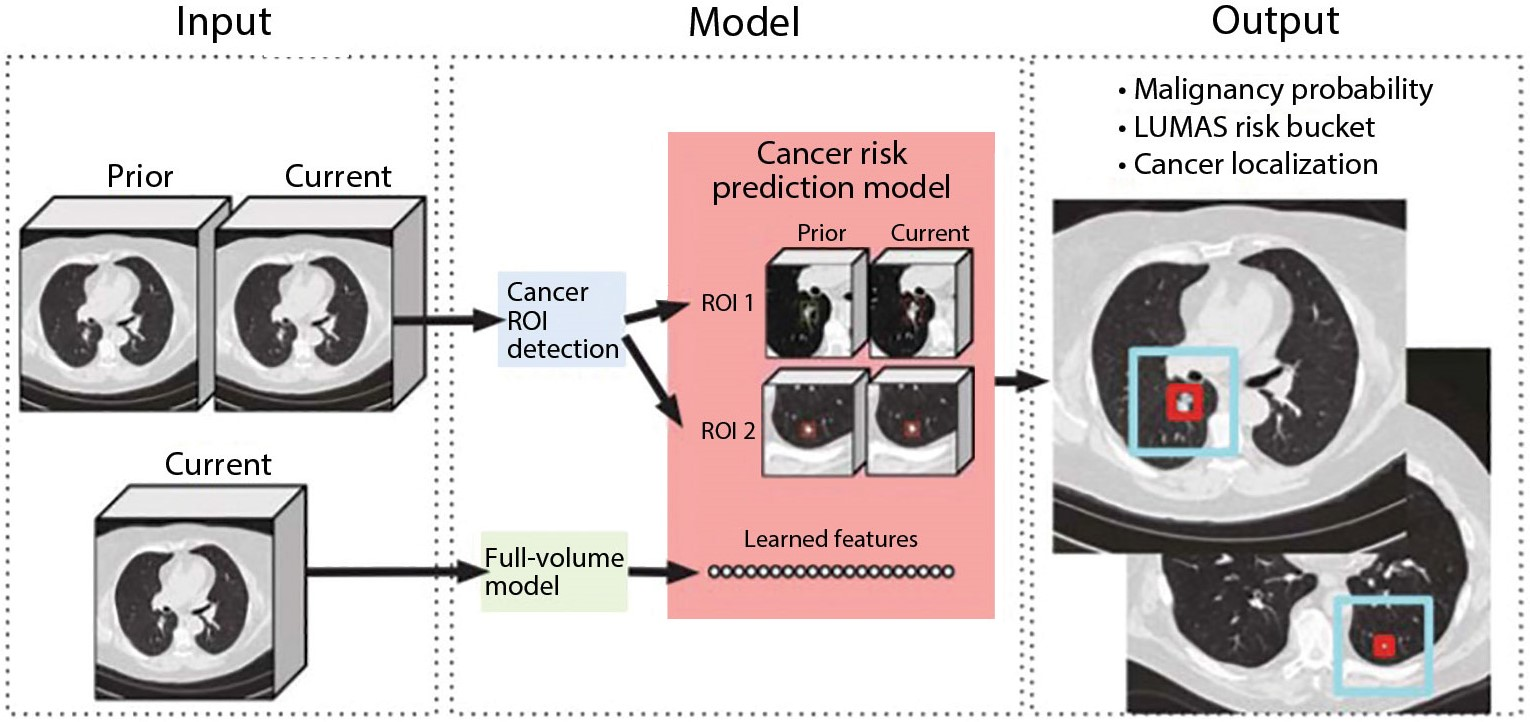
\includegraphics[width=1\linewidth]{imagenes_articulos/sp21_01} \end{center}
\figcaption{Modelo para detección de cáncer.  \ Fuente: https://goo.su/YEcqXqz}

\end{minipage}
\end {flushleft}

\textbf{Caracterización}

La caracterización es una de las etapas más amplias de la oncología, pues esta consiste en generar una descripción amplia de los tumores para detectar qué tanto se ha expandido el cáncer, si los tumores son benignos o malignos y catalogar el cáncer en etapas. Esta etapa también se extiende a la predicción de la evolución del cáncer y cómo este puede responder a distintos tratamientos, es aquí donde entran los algoritmos de deep learning.

\bigskip
\bigskip
\bigskip
\bigskip

Las redes neuronales han demostrado resultados satisfactorios al momento de predecir la agresividad de un cáncer, así como poder proponer qué opciones de tratamiento serán las más adecuadas para ese cáncer, como decidir entre un tratamiento agresivo que incluya radioterapia, cirugía y quimioterapia o esperar a la evolución de este.

\begin {flushleft}
\noindent\begin{minipage}[c]{\columnwidth}

\begin{center}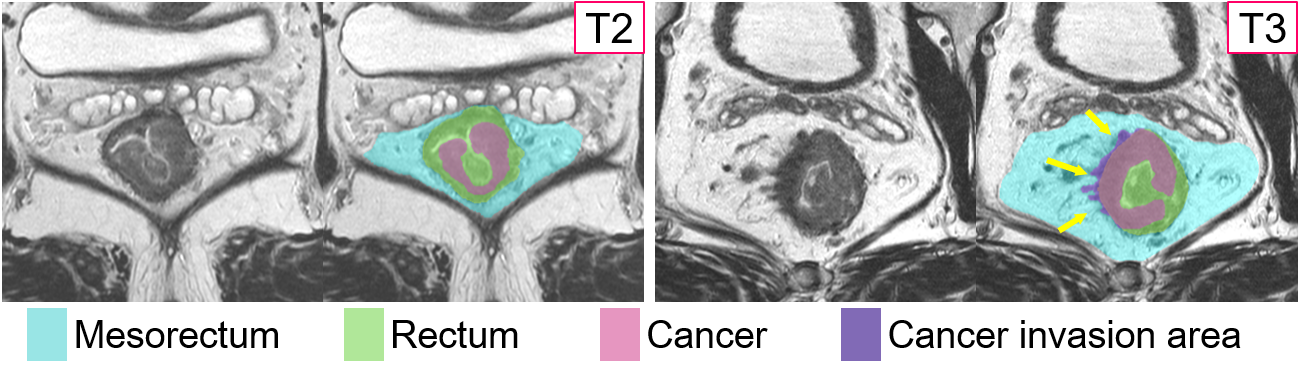
\includegraphics[width=1\linewidth]{imagenes_articulos/sp21_02} \end{center}
\figcaption{Relación entre el cáncer de recto y tejidos. 
Fuente: https://goo.su/lJlB7}

\end{minipage}
\end {flushleft}

\textbf{Monitoreo}

Por último, la fase del monitoreo se encarga de monitorear los cambios en los tumores con el paso del tiempo, ya sea por su evolución natural o en respuesta al tratamiento.

Como parte de esta etapa, la inteligencia artificial se utiliza para detectar mutaciones anormales en el cáncer que pueden no ser detectadas con facilidad en radiografías. Esto permite un mejor seguimiento de la progresión del cáncer y así ayudar a los oncólogos a prever un relapso, mientras reduce la necesidad de la realización de biopsias constantes en el paciente.

\textbf{Resultados}

El Servicio Nacional de Salud (NHS) en el Reino Unido ya está utilizando un modelo de deep learning llamado MIA entrenado para detectar síntomas tempranos de cáncer de mama.
Según la BBC, desde que se empezó a utilizar en 2023, ha sido capaz de detectar síntomas de cáncer que los doctores fueron incapaces de detectar en 11 mujeres. Modelos como MIA están en fases tempranas de desarrollo y están bastante restringidos por regulaciones, como no poder acceder al historial médico del paciente, pero con suficiente tiempo y apoyo del gobierno podrían llegar a ser herramientas indispensables para el análisis oncológico.

\begin {flushleft}
\noindent\begin{minipage}[c]{\columnwidth}

\begin{center}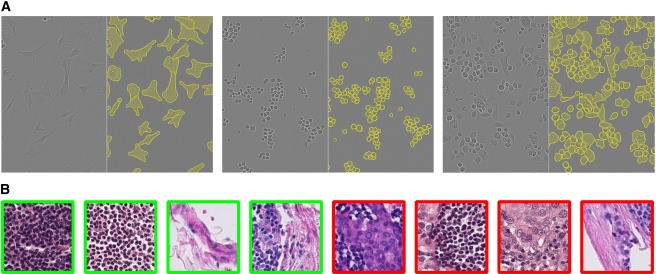
\includegraphics[width=1\linewidth]{imagenes_articulos/sp21_03} \end{center}
\figcaption{Clasificación de imágenes con MIA.
Fuente: https://goo.su/CR0L7}

\end{minipage}
\end {flushleft}

\hypertarget{conclusiones}{%
\section{Conclusiones}\label{conclusiones}}

El deep learning se compone de algoritmos que intentan imitar el comportamiento humano, entre estos algoritmos, el más utilizado actualmente es el reconocimiento de imágenes. Una de las áreas en las cuales se ha visto el potencial del algoritmo de reconocimiento de imágenes es en la Oncología y son usados, en concreto, para tres tareas indispensables al momento de tratar a un paciente con cáncer. Emplear un algoritmo de reconocimiento de imágenes al momento de realizar un diagnóstico sobre una persona puede reducir el error humano, evitando que existan falsos negativos. Este tipo de tecnologías no se limita solamente identificar posibles cánceres, sino también la gravedad de los mismos (que tan avanzados se encuentran), realizar predicciones acerca de su evolución y realizar monitoreos sobre la evolución que estos puedan tener a lo largo del tiempo.

\hypertarget{referencias}{%
\section{Referencias}\label{referencias}}

\begin{itemize}
\item
  {[}1{]} Bhinder, B., Element, O, Gilvary, C. y Madhukar, N. ``Artificial Intelligence In Cancer Research And Precision Medicine''. Cancer Discovery, 1 de abril de 2021. Accedido el 29 de julio de 2024. \url{https://doi.org/10.1158/2159-8290.cd-21-0090}
\item
  {[}2{]} Bi, W., Birkbak, Ni. J., Giger, M. L., Hosny, A., Schabath, M. B., et al.~``Artificial Intelligence In Cancer Imaging: Clinical Challenges And Applications''. CA A Cancer Journal For Clinicians, 5 de febrero de 2019. Accedido el 29 de julio de 2024.
  \url{https://doi.org/10.3322/caac.21552}
\item
  {[}3{]} Cancer Research UK. ``Why Is Early Cancer Diagnosis Important?'', 30 de marzo de 2023. Accedido el 29 de julio de 2024.
  \url{https://goo.su/q1mPJas}
\item
  {[}4{]} Kleinman, Zoe . ``NHS AI test spots tiny cancers missed by doctors''. BBC, 20 de marzo de 2024. Accedido el 09 de septiembre de 2024.
  \url{https://goo.su/lbPSt}
\end{itemize}

\end {multicols}

\medskip

\hypertarget{pareja62}{%
\chapter{Un futuro brillante con asistentes virtuales impulsados por IA}\label{pareja62}}

\begin{center}
\includegraphics[width=1\linewidth]{autores/pareja62_01} \end{center}

\begin {multicols}{2}

\textbf{\emph{Palabras clave:}} Inteligencia artificial, Asistentes virtuales, ChatGPT, Siri, Apple.

\hypertarget{introducciuxf3n-1}{%
\section{Introducción}\label{introducciuxf3n-1}}

Actualmente nos encontramos presenciando el auge y establecimiento de la inteligencia artificial en nuestras actividades cotidianas desde darnos respuesta a preguntas básicas hasta analizar y resolver problemas muy específicos siempre y cuando se le proporcione la información necesaria. Un interesante uso de la inteligencia artificial es la creación de asistentes virtuales capaces de realizar tareas como leer mensajes, tomar dictados, realizar llamadas en nuestros dispositivos de manera inmediata y sencilla para el usuario.

Podemos definir a un asistente como un individuo que ofrece ayuda, acompañamiento, atención o algún servicio hacia otras personas. Ahora, un asistente virtual es un programa de software que se utiliza en tecnologías de procesamiento de lenguaje natural (NLP) para seguir distintos comandos de voz y texto y concretar distintas o solamente una tarea específica.

\hypertarget{artuxedculo-1}{%
\section{Artículo}\label{artuxedculo-1}}

En la búsqueda de facilitar las tareas diarias de las personas, se han creado diferentes asistentes virtuales como Siri, Alexa, Cortana y el Asistente de Google, con el paso del tiempo estos asistentes han ido evolucionando para entender de mejor manera el lenguaje natural y realizar funciones con mayor complejidad, respondiendo preguntas y realizar tareas específicas.

Con el avance tecnológico, fue necesario integrar inteligencia artificial en estos asistentes para aumentar significativamente su capacidad de respuesta. Un asistente con IA no solo mejora la respuesta ante el procesamiento del lenguaje humano sino que también mejora la experiencia del usuario al poder automatizar tareas repetitivas, realizar tareas relacionadas con Internet of Things en el cual se involucran dispositivos conectados a la red wifi que el asistente puede controlar y generar rutinas de ejecución automática.

La ventaja de un asistente móvil está en su portabilidad, llevar un asistente a todos lados en nuestro bolsillo representa grandes ventajas como activar en remoto todos nuestros dispositivos desde nuestro asistente personal de bolsillo y permitiendo organizar nuestro día de una mejor manera e inmediatamente.

Un asistente virtual que implementa un modelo de Inteligencia artificial en una empresa marca una gran diferencia en la forma de interactuar con sus clientes, ya que puede ofrecer una disponibilidad al cliente de tiempo completo sin la intervención del factor humano, representando una mejor experiencia para el usuario, también puede recopilar y realizar
análisis de datos de interacciones con los usuarios, proporcionando información valiosa para la mejora de productos o servicios.

\begin {flushleft}
\noindent\begin{minipage}[c]{\columnwidth}

\begin{center}
\includegraphics[width=1\linewidth]{imagenes_articulos/sp62_01} \end{center}
\figcaption{Iphone Siri. Fuente: https://goo.su/3xyqgV}

\end{minipage}
\end {flushleft}

Si nos enfocamos en el futuro de los asistentes virtuales con base en Apple, observamos que se ha estado trabajando fuertemente en integrar la inteligencia artificial en sus productos. Esto se refleja en las nuevas mejoras de sus funciones como Siri, en la cámara y en otras áreas. Está a la puerta su nuevo gran paso, en el cual se ha incorporado inteligencia artificial a sus últimos modelos de iPhone llamado Apple Intelligence. Esta nueva tecnología permitirá una personalización avanzada y una mejora significativa en el asistente virtual Siri.

\bigskip
\bigskip

Con Apple Intelligence, se pueden generar distintos tipos de contenido como textos, traducciones y hasta imágenes. A diferencia de otros asistentes virtuales hoy en día, la IA de Apple está restringida para respetar la privacidad de sus usuarios al no compartir datos personales con terceros. Esta característica es una medida a las crecientes preocupaciones sobre la privacidad y la seguridad de los datos en el mundo digital actual. En el futuro la apuesta de Apple por una IA más segura y privada podría marcar una tendencia en la industria tecnológica.

A su vez también tenemos los avances de Microsoft en Microsoft Copilot nos facilita y nos brinda soluciones en actividades como por ejemplo escribir correos electrónicos, generar ideas de presentaciones, escribir código para los programadores entre otros usos. Se espera que Microsoft incluya más tecnología de IA en sus sistemas operativos en un futuro haciendo más sencillas las tareas.

\hypertarget{conclusiones-1}{%
\section{Conclusiones}\label{conclusiones-1}}

Hoy en día, los asistentes virtuales impulsados por inteligencia artificial representan una revolución tecnológica. Estos asistentes generan respuestas más rápidas y comprenden mejor el lenguaje humano y tienen una mejor comprensión del lenguaje humano. Estos asistentes nos facilitan el día a día con las tareas cotidianas como lo pueden ser el control de dispositivos del hogar y la gestión de agendas, también tienen un impacto muy positivo en la calidad de vida de sus usuarios. Conforme la tecnología avance, se espera que estas herramientas sean aún más eficaces y personalizables, permitiendo que el usuario tenga un asistente que responda a sus necesidades específicas. Como se destacó en el artículo la privacidad será un factor crucial a tomar en cuenta cuando se trata de elegir un asistente
virtual en un mundo donde todo está digitalizado.

\hypertarget{referencias-1}{%
\section{Referencias}\label{referencias-1}}

\begin{itemize}
\item
  {[}1{]} Cahun, Antonio.``Apple aplicó un Te pago con promoción a OpenAI en la alianza por integrar ChatGPT en iPhone'', Xataka México, 13 de junio 2024, acceso el 1 de agosto de 2024. \url{https://goo.su/BkdnU}
\item
  {[}2{]} Icrono. ``Cómo crear un asistente virtual con inteligencia artificial para empresas'', Anaimo, 9 de julio de 2024, acceso el 31 de julio de 2024. \href{https://anaimo.com/como-crear-un-asistente-virtual-con-inteligencia-artificial-para-empresas/}{https://anaimo.com}
\item
  {[}3{]} Quispe Alarcón, Gianfranco. ``El Chat GPT actual no corrobora la información'', Universidad de Piura, 12 de junio 2023, acceso el 1 de agosto de 2024.
  \href{https://www.udep.edu.pe/hoy/2023/06/el-chat-gpt-actual-no-corrobora-la-informacion/}{https://www.udep.edu.pe}
\end{itemize}

\end {multicols}

\medskip

\HRule

\medskip

\hypertarget{pareja43}{%
\chapter{Revolución en IA: Herramientas y plataformas clave para desarrolladores}\label{pareja43}}

\begin{center}
\includegraphics[width=1\linewidth]{autores/pareja43_01} \end{center}

\begin {multicols}{2}

\textbf{\emph{Palabras clave:}} Modelos predictivos, Inteligencia Artificial, Algoritmos de aprendizaje automático, Redes neuronales, Automatización, Análisis de datos.

\hypertarget{introducciuxf3n-2}{%
\section{Introducción}\label{introducciuxf3n-2}}

La inteligencia artificial (IA) está revolucionando el desarrollo de software y transformando numerosas industrias, desde la salud hasta las finanzas. Esta transformación es impulsada por herramientas y plataformas que facilitan el desarrollo, entrenamiento y despliegue de modelos de IA, democratizando el acceso a tecnologías avanzadas.

En este artículo, explicaremos las herramientas y plataformas clave que están impulsando esta revolución, destacando sus características, impacto y aplicaciones prácticas. Nuestro objetivo es proporcio-
nar una guía detallada para que los desarrolladores puedan aprovechar estas tecnologías, creando soluciones innovadoras y eficientes.

\hypertarget{artuxedculo-2}{%
\section{Artículo}\label{artuxedculo-2}}

Las Nuevas Herramientas de IA
Ante la necesidad de las empresas de automatizar y agilizar sus procesos, nuevas herramientas han surgido con el apoyo de la inteligencia artificial, las cuales están dando el siguiente paso en la transformación digital para estas empresas, desde el famoso GPT-4 para la creación de contenido, que ha revolucionado la generación del mismo y ha demostrado gran adaptación para las necesidades de diferentes empresas, hasta inteligencias artificiales para la analítica predictiva ayudando a predecir comportamientos y tendencias futuras con el uso de los datos.

Así mismo, en el sector sanitario tenemos a Cori, una inteligencia artificial enfocada a ser un asesor de salud para las personas con diabetes. Este es uno de esos casos de uso en lo que podemos ver la gran diversidad de aplicaciones posibles de la inteligencia artificial las cuales también podemos ver como una oportunidad para crear tecnologías útiles e innovadoras.

\begin {flushleft}
\noindent\begin{minipage}[c]{\columnwidth}

\begin{center}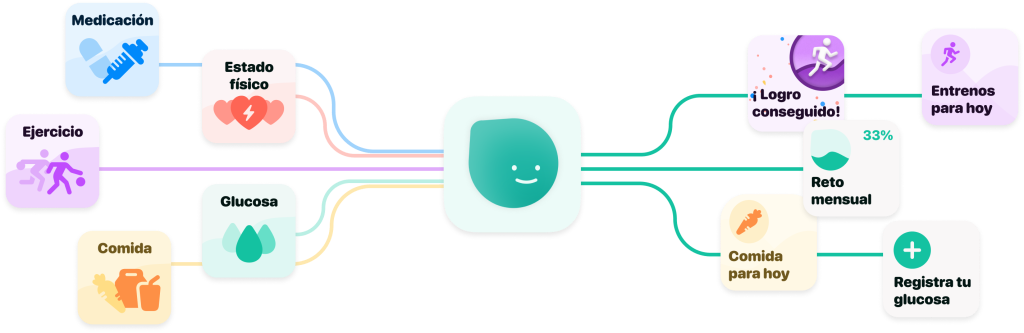
\includegraphics[width=1\linewidth]{imagenes_articulos/sp43_01} \end{center}
\figcaption{El entrenador personal para tu diabetes.
Fuente: https://cori.care/es/}

\end{minipage}
\end {flushleft}

\textbf{Plataformas de IA y su impacto en el desarrollo de soluciones empresariales}

Las herramientas y plataformas de IA están en constante evolución, incorporando nuevas funcionali-
dades y mejoras para facilitar el desarrollo y la implementación de modelos de IA.Con el auge de la inteligencia artificial, ha sido necesario encontrar herramientas que puedan simplificar y acelerar este proceso.

Una de las más comunes es Scikit-learn, una biblioteca de código abierto construida sobre otras librerías de Python como NumPy, SciPy, y matplotlib. Scikit-learn es ideal para análisis de datos predictivo, aprendizaje supervisado y no
supervisado, ofreciendo una amplia gama de algoritmos que permiten a los desarrolladores construir modelos de machine learning de manera eficiente.

Además de Scikit-learn, existen otras plataformas robustas que han tenido un impacto significativo en el desarrollo de soluciones empresariales:

\begin{itemize}
\item
  \textbf{TensorFlow:} Es una librería de código libre para Machine Learning desarrollada por Google, diseñada para construir y entrenar redes neuronales artificiales que detectan patrones y razonamientos similares a los humanos.
\item
  \textbf{PyTorch:} Es un marco de aprendizaje profundo de código abierto desarrollado por Facebook AI Research con una API de alto nivel basada en Python. Conocido por su flexibilidad y facilidad de uso, PyTorch es popular en la academia y la investigación. Admite diversas estructuras de redes neuronales y permite la creación y ejecución eficiente de modelos de aprendizaje profundo.
\end{itemize}

\medskip
\medskip
\medskip

\begin{itemize}
\tightlist
\item
  \textbf{Microsoft Azure AI:} La plataforma de IA de Microsoft Azure ofrece una amplia gama de servicios y herramientas para el desarrollo de soluciones de inteligencia artificial, desde servicios de machine learning hasta herramientas de análisis cognitivo.
\end{itemize}

Estas plataformas no solo facilitan el desarrollo de modelos de IA, sino que también permiten a las empresas implementar soluciones de IA escalables y eficientes. Al proporcionar herramientas integradas para el análisis de datos, entrenamiento de modelos, y despliegue en producción, estas plataformas están transformando la manera en que las empresas operan, permitiéndoles aprovechar el poder de la inteligencia artificial para innovar y mantenerse
competitivas en un mercado en constante cambio.

\textbf{Tendencias futuras}

El futuro de las herramientas y plataformas de IA está marcado por innovaciones como el aprendizaje federado, que permite entrenar modelos sin compartir datos, mejorando la privacidad y seguridad. La integración de IA con el Internet de las Cosas (IoT) y las mejoras en la infraestructura de edge computing están impulsando la creación de sistemas más inteligentes y autónomos, lo que promete revolucionar aún más diversas industrias y aplicaciones.

\hypertarget{conclusiones-2}{%
\section{Conclusiones}\label{conclusiones-2}}

Las herramientas y plataformas de inteligencia artificial, como Scikit-learn, TensorFlow y PyTorch, han revolucionado diversos sectores al automatizar y optimizar procesos clave. Para los desarrolladores, estas herramientas son fundamentales, ya que ofrecen marcos de trabajo robustos y flexibles para construir y entrenar modelos de aprendizaje automático y redes neuronales, lo que facilita la implementación de soluciones de alta calidad. Estas tecnologías permiten desarrollar modelos avanzados para analizar datos, predecir tendencias y personalizar servicios. Al facilitar la creación de soluciones adaptadas a las necesidades específicas de cada industria, la inteligencia artificial está transformando la manera en que las empresas operan y generan valor, expandiendo continuamente las oportunidades de
innovación.

\hypertarget{referencia}{%
\section{Referencia}\label{referencia}}

\begin{itemize}
\item
  {[}1{]} Alliax. La inteligencia artificial (IA) y su rol en las soluciones empresariales modernas. 2023.
  \href{https://www.alliax.com/la-inteligencia-artificial-ia-y-su-rol-en-las-soluciones-empresariales-modernas/}{https://www.alliax.com}
\item
  {[}2{]} Bergmann, Dave. Stryker, Cole. ``¿Qué es PyTorch?''. IBM. 2024. \href{https://www.ibm.com/mx-es/topics/pytorch\#:~:text=PyTorch\%20es\%20un\%20marco\%20de,alto\%20nivel\%20basada\%20en\%20Python\%20}{https://www.ibm.com/}
\item
  {[}3{]} Jon Larkin Alonso. ``¿Qué es TensorFlow y para qué sirve?''. Incentro. 2022.
  \url{https://www.incentro.com/es-ES/blog/que-es-tensorflow}
\item
  {[}4{]} Ramírez, Lorena. ``Herramientas y aplicaciones de Inteligencia Artificial que tu empresa necesita'' IEBS School (blog). 6 de febrero de 2024.
  \href{https://www.iebschool.com/blog/herramientas-aplicaciones-inteligencia-artificial-big-data/}{https://www.iebschool.com}
\item
  {[}5{]} Scikit-Learn. ``User Guide'' scikit-learn. 2024. \url{https://scikit-learn.org/stable/user_guide.html}
\end{itemize}

\end {multicols}

\medskip

\HRule

\medskip

\hypertarget{pareja65}{%
\chapter{Uso de herramientas de código abierto en la detección de fraudes: Implementación de PyTorch en el sector financiero de Guatemala}\label{pareja65}}

\begin{center}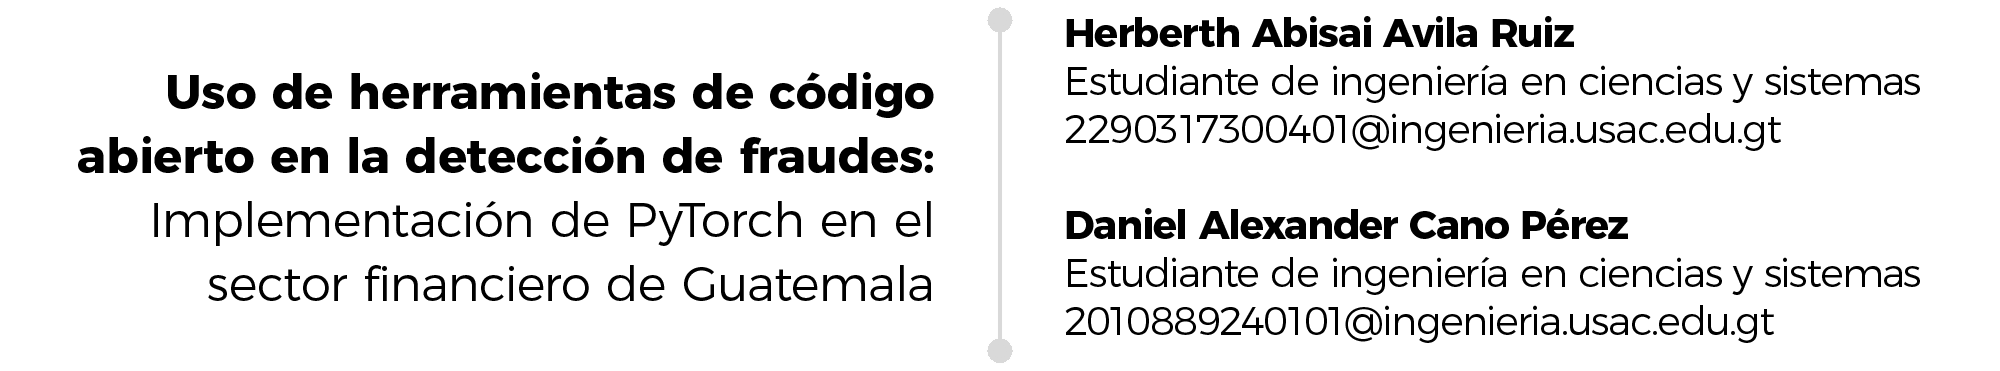
\includegraphics[width=1\linewidth]{autores/pareja65_01} \end{center}

\begin {multicols}{2}

\textbf{\emph{Palabras clave:}} Fraudes, Inteligencia artificial, Aprendizaje automático, Innovación.

\hypertarget{introducciuxf3n-3}{%
\section{Introducción}\label{introducciuxf3n-3}}

En Guatemala es muy escuchado en redes sociales o medios de comunicación un problema que ha aumentado en los últimos años, como los fraudes y anomalías dentro del sector financiero. Es fundamental abordar este problema utilizando tecnologías de última generación, como lo es la inteligencia artificial, para que tanto la industria financiera como la
población en general puedan disminuir este problema el cual ha afectado a todos.

PyTorch es una biblioteca de aprendizaje profundo que proporciona herramientas avanzadas para implementar algunos modelos de detección de anomalías y fraudes. El cual ha sido aprovechado en otros países en distintos sectores. Al aplicar esta tecnología puede ayudar a resolver un problema en el campo financiero, ya que los delitos de esta índole han aumentado considerablemente, debido a la corrupción que azota el país.

\hypertarget{artuxedculo-3}{%
\section{Artículo}\label{artuxedculo-3}}

\textbf{Análisis en otros países}

Este framework ha sido ampliamente utilizado en varios países debido a sus capacidades de aprendizaje automático y su naturaleza de código abierto, lo que brinda una gran flexibilidad y facilidad de uso. Además, cuenta con un fuerte apoyo proporcionado por la comunidad.

Entre los países que han implementado esta tecnología se encuentra los Estados Unidos, donde los bancos y las compañías de tarjetas de crédito siempre están buscando métodos más sofisticados para detectar y prevenir el fraude. El uso de esta herramienta ha sido particularmente beneficioso debido a su capacidad para procesar grandes cantidades de datos
y crear modelos complejos de aprendizaje automático.

Las aplicaciones que se encuentran en el sector financiero son las siguientes:

\begin{itemize}
\item
  \textbf{Redes neuronales recurrentes (RNN):} para analizar series temporales de datos de transaccio-
  nes e identificar patrones secuenciales que podrían indicar actividad fraudulenta.
\item
  \textbf{Redes neuronales convolucionales (CNN):} para el procesamiento de imágenes. Las CNN se utilizan ahora para identificar patrones en datos tabulares de transacciones, mejorando así la precisión de la detección de fraude.
\end{itemize}

Uno de los bancos más grandes del mundo, JPMorgan Chase, utiliza PyTorch para analizar grandes cantidades de datos financieros. Los modelos que implementan pueden detectar al instante patrones y comportamientos poco usuales, lo que permite responder lo más rápido posible para prevenir el fraude. Por ejemplo, pueden identificar transacciones que difieren de los patrones de gasto comunes de un cliente, lo que indica un posible fraude.

\textbf{Situación en Guatemala}

En el país, la detección de fraudes financieros aún enfrenta muchos desafíos. En los últimos años, ha habido un aumento significativo en los delitos financieros, convirtiéndose en un problema potencialmente incontrolable. Entre los casos más conocidos están la evasión fiscal y el lavado de dinero. En el país aún se utilizan métodos de detección de fraudes tradicionales en su mayoría, como la revisión manual de información, la verificación de identidad y el monitoreo de transacciones.

Una de las principales razones del incremento en los casos relacionados con el fraude es la corrupción, que en los últimos años se ha vuelto una práctica común en el país. Además, la falta de interés y acción por parte de las instituciones de justicia ha permitido que muchos de estos casos queden impunes. Por otra parte, la educación financiera entre la ciudadanía es limitada o casi inexistente, lo que aumenta el riesgo de ser víctima de estafas, fraudes o robo de identidad.

\bigskip
\bigskip
\bigskip
\bigskip

\textbf{¿Cómo implementarlo en Guatemala?}

En Guatemala utilizando PyTorch se podrían utilizar para desarrollar modelos de aprendizaje automático que analicen transacciones en tiempo real. Estos modelos pueden incluir redes neuronales recurrentes (RNN) y redes neuronales convolucionales (CNN) para detectar patrones anómalos y actividades sospechosas. Esto no solo aumentaría la seguridad en el sector financiero, sino también la confianza de los clientes, ya que ayudaría a prevenir fraudes y reducir las pérdidas económicas tanto para las instituciones como para sus usuarios.

\textbf{Retos}

Al momento de que se quiera implementar este framework, es importante tomar en cuenta los retos que puede llevar su implementación los cuales son lo siguientes:

\begin{enumerate}
\def\labelenumi{\arabic{enumi}.}
\item
  Uno de esos sectores donde se puede aprovechar mejor es en el sector justicia, pero debido a la corrupción presente en el país, esto puede llegar a ser un problema para los intereses de diferentes instituciones, ya que podría evitar los excesivos casos de lavado de dinero.
\item
  La resistencia al cambio, es un factor muy crítico en el país, esto debido a la cultura que llega a ser muy conservadora, provocando que no se logre adaptar al entorno guatemalteco, debido a que la sociedad está tan acostumbrada a métodos ortodoxos y prefiere evitar cualquier cambio en su entorno.
\end{enumerate}

\hypertarget{conclusiones-3}{%
\section{Conclusiones}\label{conclusiones-3}}

La implementación de PyTorch en el sector financiero de Guatemala ofrece numerosos beneficios, incluyendo la mejora en la detección de fraudes en tiempo real y la reducción de pérdidas financieras. Es crucial tomar acciones en contra de estos delitos, debido a su aumento en la población guatemalteca, Con estas medidas se busca que no solo los bancos
sean beneficiados para no contar con pérdidas, ya que al aumentar la seguridad de las transacciones, fortalecer la confianza los clientes, mejorando así la fidelidad y satisfacción general.

\hypertarget{referencias-2}{%
\section{Referencias}\label{referencias-2}}

\begin{itemize}
\item
  {[}1{]} ''Anomaly Detection in Financial Data with PyTorch - Fouad Roumieh Medium.'',Roumieh, F., 20 de octubre 2023, \url{https://acortar.link/6dklLC}
\item
  {[}2{]} ''Delitos financieros en Guatemala: Análisis de la situación actual'', Declaraguate Omisos, 30 de enero 2024, \url{https://acortar.link/B4zpse}
\item
  {[}3{]} ''JPMorgan Chase using advanced AI to detect fraud. American Banker'', Crosman, P. 22 de diciembre 2023, \url{https://acortar.link/VGutC0}
\item
  {[}4{]} ''PyTorch. Enterprise AI.'', Yasar, K., \& Lewis, S., 16 de noviembre 2022, \url{https://acortar.link/w0YCrw}
\item
  {[}5{]} ''PyTorch 2.4 documentation. (s.f.)'', PyTorch documentation,2023, \url{https://acortar.link/PqmwUz}
\end{itemize}

\end {multicols}

\medskip

\HRule

\medskip
%%%%%% SECCION 2 
\includepdf{images/seccion2.pdf}

\AddEverypageHook{%
\ifthenelse{\value{page}<27}%
{\ifthenelse{\isodd{\value{page}}}%
  	{\backgroundsetup{scale=1, color=white, opacity=1, angle=0, contents={
\includegraphics[width=\paperwidth,height=\paperheight]{latex/background_numberimpar.pdf}}}}%
  	{\backgroundsetup{scale=1, color=white, opacity=1, angle=0, contents={
\includegraphics[width=\paperwidth,height=\paperheight]{latex/background_numberpar.pdf}}}}%
}{}%
\BgMaterial}
%%%%%%%%%%%%%%%%%%%%%%%%%%%
\hypertarget{chaac}{%
\chapter{Ganadores RIIC 4.0 Categoría Senior: Equipo Chaac}\label{chaac}}

\begin{center}
\includegraphics[width=1\linewidth]{autores/pareja00_chaac} \end{center}

\begin {multicols}{2}

\hypertarget{entrevista-1}{%
\section{Entrevista}\label{entrevista-1}}

\textbf{¿Qué es el Rally Interdepartamental de Innovación 4.0 (RIIC 4.0)?}

Es una competencia iniciada en 2021 que invita a estudiantes a formar grupos y resolver problemas comunitarios mediante tecnologías 4.0, principalmente el Internet de las Cosas (IoT). Inspirada en la industria 4.0 de Alemania, busca aplicar estas innovaciones en Guatemala para abordar diversos desafíos.

\textbf{¿Cómo se enteraron del Rally Interdepartamental de Innovación 4.0 (RIIC 4.0)?}

En 2022, Estuardo, junto con Fernanda y Francisco, se enteraron de la competencia a través de redes sociales. Habían participado anteriormente en un programa de becas y, motivados por esa experiencia, decidieron trabajar juntos en una solución. Además, Estuardo fue contactado por SENACYT, lo que también contribuyó a su conocimiento sobre la competencia.

\textbf{¿En qué consiste el Rally Interdepartamental de Innovación 4.0?}

El Rally es una competencia interdepartamental en la que grupos de jóvenes multidisciplinarios proponen soluciones tecnológicas a problemas en el país. A medida que avanzan las fases, se seleccionan los grupos con las mejores propuestas. Al final, se evalúan la presentación de un prototipo y su viabilidad, culminando con la premiación de los ganadores.

\textbf{¿Qué los ha motivado a participar en el Rally Interdepartamental de Innovación? 4.0?}

Fernanda destaca que una de las motivaciones para participar en el Rally es la oportunidad de crear y aplicar los conocimientos adquiridos en la universidad en proyectos significativos. Además, valora que el Rally tiene como objetivo beneficiar a la comunidad, lo que resulta gratificante al poder contribuir al desarrollo social. La posibilidad de que sus ideas evolucionen de simples prototipos a proyectos reales que generen beneficios para diversas comunidades es también un aspecto inspirador para el equipo.

\textbf{¿Qué criterios se toman en cuenta para su participación y premiación?}

Francisco explica que el Rally comienza con una fase de capacitación en la que los equipos deben presentar avances y demostrar la viabilidad de sus proyectos. Aquellos que identifican claramente el problema a resolver avanzan y reciben un kit para desarrollar su prototipo. Luego, presentan cómo funcionará su proyecto, y los prototipos más funcionales pasan a la final.

La evaluación final considera tanto el tiempo y dedicación como el desarrollo y viabilidad del proyecto. En su primera participación, el equipo destacó por realizar un análisis económico, lo que se convirtió en un criterio de evaluación en la segunda edición, en 2023. En resumen, los principales criterios de evaluación y premiación son la funcionalidad, dedicación y viabilidad del proyecto.

\textbf{¿Cómo se conformó el equipo?}

Estuardo menciona que él, Francisco y Fernanda son exbecarios de un programa del Departamento de Estado de 2022, donde se conocieron y aprendieron sobre el trabajo interdisciplinario. En su primera participación, su grupo fue único en contar con estudiantes de diferentes áreas, como ingeniería ambiental y sistemas de producción agrícola. En 2023, decidieron diversificar la carga de trabajo al integrar a Carlos, estudiante de ingeniería mecatrónica, lo que permitió desarrollar un proyecto más completo. Esto les permitió a cada uno enfocarse en sus fortalezas.

\textbf{¿De qué se trata el proyecto Farmflow?}

Farmflow nació con el objetivo de llevar tecnología a comunidades pequeñas para optimizar ciertas variables, y finalmente desarrolló una copla universal para drones. Este dispositivo, adaptable a cualquier dron básico, reduce los costos de alquiler, permitiendo la recolección de datos que se almacenan en una base de datos para diversos procesos. El diseño de la copla fue versátil y accesible, pensada para que tanto grandes empresas como comunidades pequeñas pudieran beneficiarse.

Durante el desarrollo, el equipo enfrentó limitaciones técnicas, pero logramos integrar el sistema para que este fuese funcional. Se descubrió que la copla tenía aplicaciones amplias, incluyendo la prevención de desastres naturales y la gestión de recursos hídricos y agrícolas.

El proyecto se orientó hacia una inversión única por copla, con costos mensuales para servicios en la nube. Se realizó un análisis de costos para asegurar que el proyecto fuera autofinanciable y sin fines de lucro, beneficiando a pequeños agricultores e instituciones gubernamentales a un costo bajo.

\textbf{¿Cómo surgió la idea del proyecto?}

Francisco explica que el equipo se enfocó en problemáticas comunes que afectan a comunidades vulnerables en Guatemala, especialmente ante los desastres climáticos, como inundaciones y derrumbes, que han causado muchas pérdidas humanas y económicas. Decidieron concentrarse en la región de Alta Verapaz, aunque su solución es aplicable a todo el país. A medida que desarrollaron el proyecto, se dieron cuenta de su potencial económico y su capacidad para contribuir a la prevención de desastres naturales y pérdidas en la agricultura, beneficiando así tanto a las personas como a la economía agrícola.

\textbf{¿Qué roles desempeñaron en el desarrollo del proyecto?}

Los roles del equipo se distribuyeron según las especializaciones de cada miembro. Estuardo lideró el área de software y fue el enlace que organizó al grupo, ayudando a definir las variables de medición y costos. Carlos se encargó del hardware, incluyendo la impresión 3D y la electrónica, mientras que Estuardo montó la arquitectura de datos desde el Raspberry Pi a Azure IoT Services y creó una aplicación en Power Apps para visualizar la información en Cosmos DB. Francisco se ocupó de las variables de Atterberg y su aplicación en el proyecto, y Fernanda desarrolló el modelo de negocios con un enfoque social, lo que fue clave para la selección del proyecto. Estuardo destacó la importancia del trabajo interdisciplinario, señalando que, como estudiantes de sistemas, a menudo no conocen los problemas en otras áreas que podrían ayudar a resolver.

\textbf{¿Qué herramientas aplicaron para llevar a cabo el proyecto?}

El equipo comenzó utilizando Orange Pi, pero enfrentó dificultades por la falta del sistema operativo necesario para integrar datos con Azure. Por ello, se cambió a Raspberry Pi, empleando la arquitectura de referencia de Azure IoT. Los datos se enviaron desde Raspberry Pi a Azure IoT Hub y se procesaron mediante Azure Stream Analytics, permitiendo su visualización en Excel y la creación de un prototipo con Power Apps, aunque se consideró costoso para una pequeña empresa.

En cuanto al hardware, además del Orange Pi, se utilizaron sensores para medir humedad y temperatura del suelo. Se exploró la posibilidad de usar una cámara con inteligencia artificial para analizar riesgos de desastres naturales, pero las dificultades con el Orange Pi complicaron esta parte.

El equipo analizó variables como la humedad del suelo y modelos climáticos, utilizando modelos estadísticos para prever eventos futuros.

En el análisis financiero, se evaluó la inversión inicial y se aplicaron indicadores como EVA y ROI para determinar el costo mínimo y el periodo de retorno de la inversión, lo que ayudaría a establecer la viabilidad económica del proyecto.

\textbf{¿Qué oportunidades y fortalezas le ven al proyecto Farmflow?}

El proyecto se destaca por su originalidad y accesibilidad en comparación con drones comerciales costosos que miden variables similares. Su bajo presupuesto lo hace viable para pequeñas economías, enfocándose en el valor social en lugar de solo en ganancias. Además, puede acoplarse a diversos drones, lo que amplía su mercado potencial.

Se identifican oportunidades de investigación interdisciplinaria, especialmente entre las facultades de agronomía e ingeniería, basándose en experiencias previas con expertos internacionales en inteligencia artificial y análisis de zonas áridas.

El proyecto, aún en fase de prototipo, tiene un gran potencial de mejora mediante inversión externa, lo que permitiría el uso de sensores más avanzados. Sin embargo, la integración de sensores de pH presenta un desafío debido a su complejidad y costo.

Finalmente, se subraya la ausencia de iniciativas similares en Guatemala, lo que representa una oportunidad significativa para entrar en un mercado aún no explorado, a diferencia de países desarrollados que ya cuentan con recursos en este ámbito.

\textbf{¿Cómo incentivar la participación en este tipo de actividades?}

Estuardo destaca que en la Escuela de Ciencias y Sistemas se está fomentando un nuevo enfoque en la presentación de proyectos, especialmente en el curso de Arquitectura de Computadoras y Ensambladores 2, donde los estudiantes buscan ideas innovadoras en IoT. Propone que se deben incentivar estas iniciativas, ofreciendo créditos extracurriculares y promoviendo el trabajo interdisciplinario, lo que ayudaría a los estudiantes a conectar su esfuerzo con resultados emotivos.

Fernanda añade que es crucial contar con un fondo de apoyo para estos proyectos, ya que los estudiantes a menudo enfrentan limitaciones económicas al invertir en materiales. Sugiere que proporcionar los recursos necesarios, como sensores y herramientas para impresiones 3D, podría eliminar barreras económicas y motivar a más estudiantes a desarrollar sus ideas.

\textbf{Mensaje final del equipo}

Estuardo enfatiza la importancia de no desmotivarse ante la falta de conocimiento, ya que se puede aprender en el camino, como él lo hizo con Cloud Services al iniciar el proyecto.

\bigskip
\bigskip

Fernanda resalta la necesidad de tener confianza en uno mismo y en el trabajo en equipo, mencionando que cada miembro aporta diferentes conocimientos, lo que potencia el resultado final. Destaca la importancia de participar en concursos y eventos, animando a otros a superar el miedo y a compartir sus ideas.

Carlos sintetiza que los pilares del éxito en un proyecto son el trabajo en equipo, la confianza, una buena gestión del tiempo y la comunicación efectiva, subrayando que las barreras son mentales y que con determinación se puede lograr cualquier objetivo.

\begin {flushleft}
\noindent\begin{minipage}[c]{\columnwidth}

\begin{center}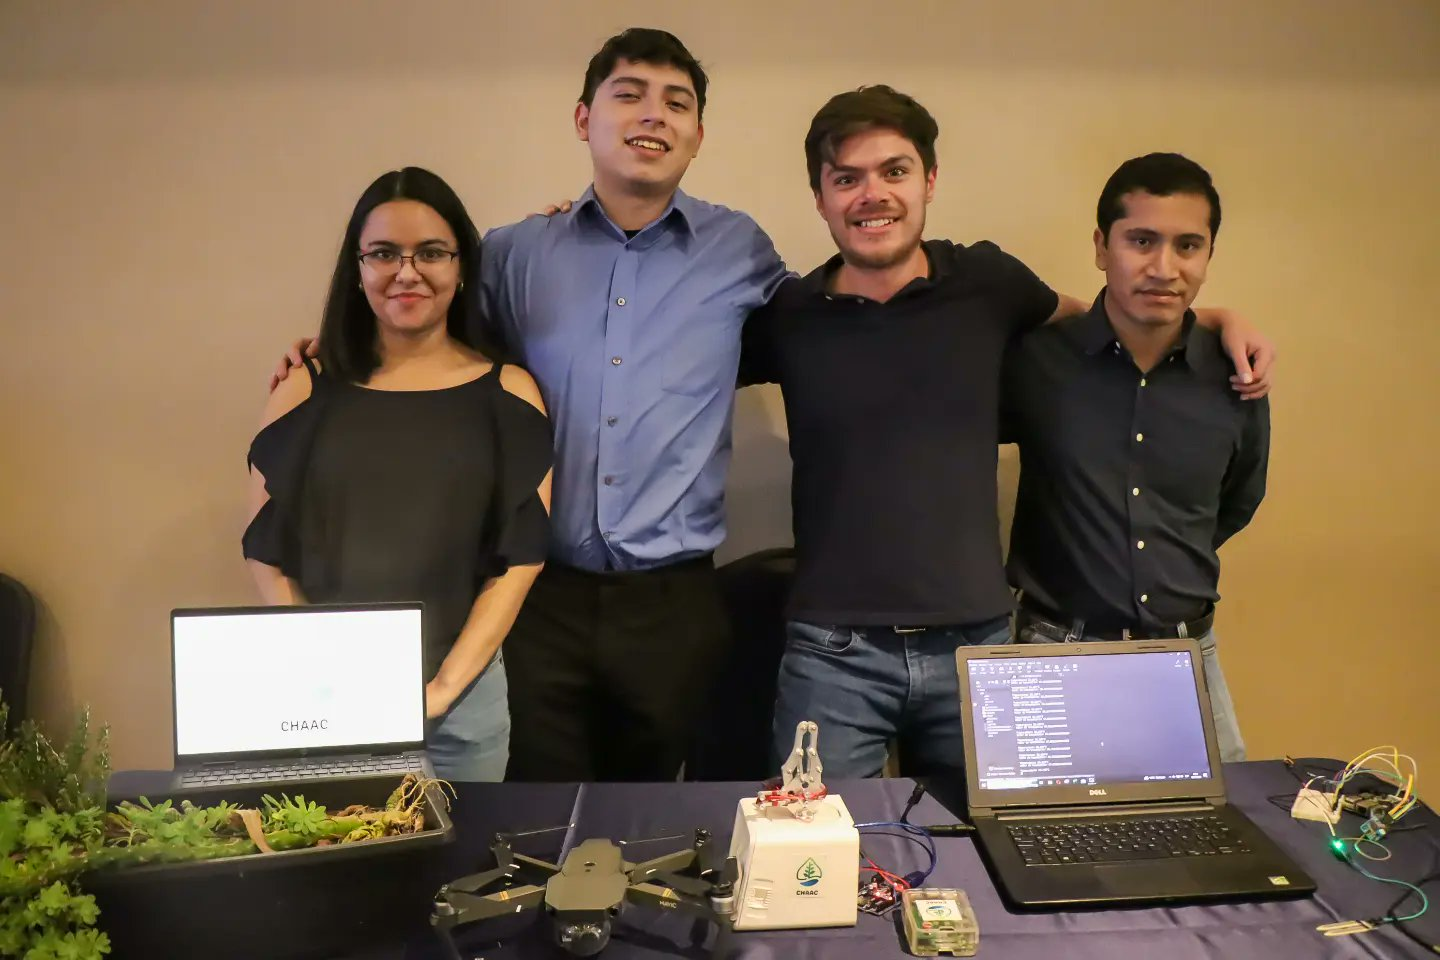
\includegraphics[width=1\linewidth]{imagenes_articulos/spchaac_01} \end{center}
\figcaption{Equipo Chaac Fuente: https://goo.su/NOWSJ7}

\end{minipage}
\end {flushleft}

\end {multicols}

\medskip

\HRule

\medskip

\hypertarget{pareja66}{%
\chapter{El Arte de la optimización de código en JavaScript: Técnicas de optimización del motor V8}\label{pareja66}}

\begin{center}
\includegraphics[width=1\linewidth]{autores/pareja66_01} \end{center}

\begin {multicols}{2}

\textbf{\emph{Palabras clave:}} JavaScript, compiladores, optimiza-
ción de código, motor V8.

\hypertarget{introducciuxf3n-4}{%
\section{Introducción}\label{introducciuxf3n-4}}

Hoy en día, JavaScript es el lenguaje que mueve la web tal y como la conocemos, pero su historia no siempre fue tan brillante. Ha evolucionado desde su nacimiento, superando una trayectoria desordenada por la falta de estandarización. El motor V8 de Google Chrome ha sido clave en este proceso además de permitir la ejecución de JavaScript en distintos entornos, más allá de los navegadores.

JavaScript ha trascendido su origen como un lenguaje de scripting básico. V8 ha incorporado mecanismos avanzados de optimización, lo que lo ha posicionado como un pilar en el ecosistema tecnológico moderno. En este artículo, se desglosan los procesos internos del motor V8, mostrando cómo hace que JavaScript sea tan eficiente y potente.

\hypertarget{artuxedculo-4}{%
\section{Artículo}\label{artuxedculo-4}}

\emph{JavaScript ha tenido una historia caótica, pero ha gozado de una acogida creciente entre los desarrolladores. Desde su prematuro nacimiento en 1995, cuando su desarrollo inicial se completó en tan solo 10 días, JavaScript careció de una especificación formal. Esto provocó que los navegadores de la época, con la urgente necesidad de establecerse como la puerta de entrada al novedoso internet, interpretaran el lenguaje de distintas maneras, etapa conocida hoy como la ``Guerra de los Navegadores''} (Rauschmayerm 2012).

Netscape, el navegador que implementó JavaScript por primera vez, solicitó en 1996 a la organización de estándares ECMA International que creara una especificación, ahora conocida como ECMA-262. Si bien fue publicado dicho estándar, el entorno que rodeaba al lenguaje seguía siendo anárquico, principalmente debido a la reticencia de Microsoft de adoptar la especificación en su navegador Internet Explorer.

Con el tiempo, la creciente capacidad y eficiencia de los navegadores modernos, especialmente Google Chrome con su motor V8, impulsaron la adopción generalizada del estándar. Estando los navegadores alineados en la misma dirección, se pudieron desarrollar características más robustas, deshaciendo la idea de que JavaScript era un lenguaje sencillo destinado solo para proporcionar interactividad básica a las páginas web.

V8 es un motor de código abierto para JavaScript y WebAssembly que ha permitido a JavaScript liberarse de su uso reservado para el navegador y ha sido adoptado en entornos de ejecución como Node.js o Deno, donde también se emplea para desarrollar aplicaciones del lado del servidor e incluso de escritorio.

La compilación es el proceso en el que el código fuente se traduce a una representación equivalente, tradicionalmente incluye varias etapas: análisis léxico, análisis sintáctico, análisis semántico, generación y optimización de código intermedio y generación de código final.JavaScript, aunque se considera un lenguaje interpretado, también involucra un proceso de compilación en el motor V8.

\begin {flushleft}
\noindent\begin{minipage}[c]{\columnwidth}

\begin{center}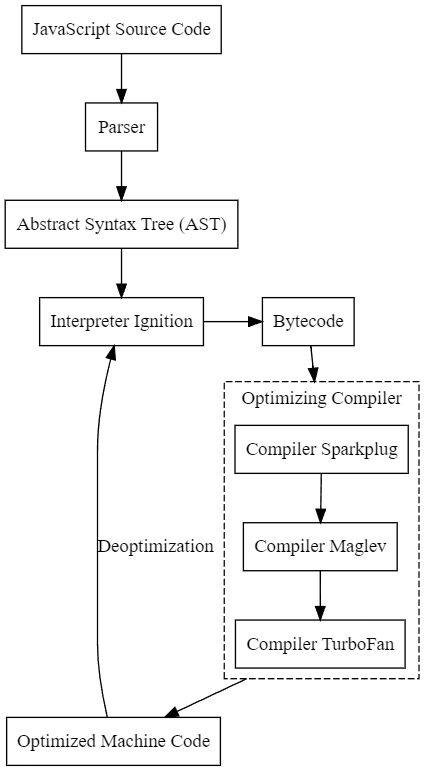
\includegraphics[width=0.47\linewidth]{imagenes_articulos/sp66_01} \end{center}
\figcaption{Arquitectura del motor V8. Fuente: Elaboración propia.}

\end{minipage}
\end {flushleft}

V8 primero analiza el texto fuente convirtiéndolo en un árbol de sintaxis abstracta (AST), una representación estructural del programa. El análisis sintáctico comienza con un escáner que procesa una secuencia de caracteres y genera tokens, bloques con significado semántico. Los tokens son consumidos por el parser de V8, que construye el AST. Desde esta etapa inicial se introducen optimizaciones, como la posibilidad de aplazar el parsing de funciones hasta que sean necesarias, técnica conocida como lazy parsing.

En lugar de ejecutar directamente las instrucciones recorriendo el AST, V8 genera una representación intermedia llamada bytecode \emph{(ver Figura 8.2)}. Bytecode es conjunto de instrucciones que se asemeja al código máquina, pero están diseñadas para ser más flexibles.
La abstracción de las instrucciones máquina en bytecode facilita la tarea del compilador y da cabida a optimizaciones. Ignition, el intérprete de V8, procesa el bytecode, lo que proporciona portabilidad a JavaScript entre plataformas, ya que el bytecode no depende de una arquitectura específica para su ejecución.

Si bien la ejecución del bytecode es relativamente eficiente, sigue siendo más lento comparado con el rendimiento de un lenguaje completamente compilado a bajo nivel. Para mejorar el rendimiento, se introduce un paso adicional,la compilación Just-In-Time (JIT).

El proceso de compilación JIT comienza cuando, en tiempo de ejecución, se detectan partes del bytecode que pueden beneficiarse de la optimización. El proceso de optimización es costoso computacionalmente, por lo V8 estima el posible beneficio comparando el tiempo de ejecución de la versión no optimizada con el que se podría obtener al optimizarla.

\begin {flushleft}
\noindent\begin{minipage}[c]{\columnwidth}

\begin{center}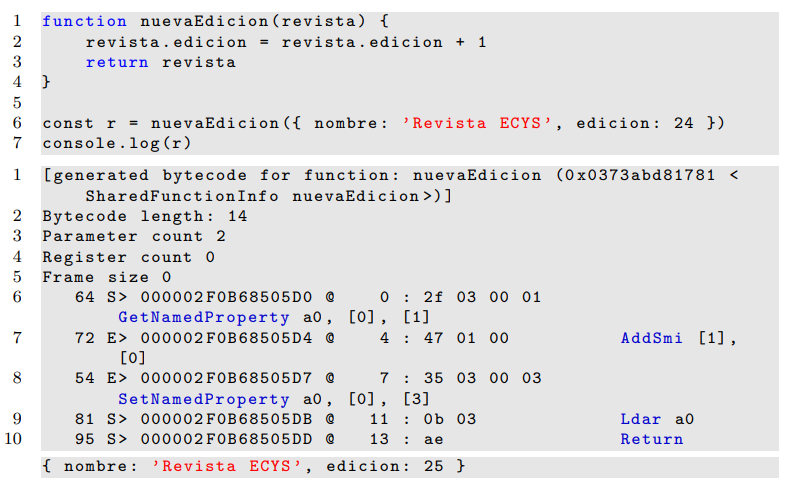
\includegraphics[width=1\linewidth]{imagenes_articulos/sp66_02} \end{center}
\figcaption{Bytecode generado por Node.js. Fuente: Elaboración propia.}

\end{minipage}
\end {flushleft}

\emph{El bytecode de las secciones identificadas como optimizables pasa por un proceso de compilación donde se pretende analizar las formas de los objetos. El compilador encargado se llama SparkPlug y es del tipo single-pass, por lo que es extremadamente rápido, si bien las optimizaciones que consigue son simples.} (Swirski 2021).

\emph{La salida de la compilación de SparkPlug es inyectada en Maglev, un compilador que emplea una representación intermedia basada en la asignación estática de una sola vez (SSA) y gráficos de flujo de control (CFG)} (Verwaest, y otros 2023).

\emph{Finalmente, la salida de las anteriores etapas llega a TurboFan, el compilador optimizador principal de V8, que utiliza una representación intermedia conocida como Sea of Nodes para realizar optimizaciones agresivas que por último son convertidas a código máquina} (Titzer 2015).

\hypertarget{conclusiones-4}{%
\section{Conclusiones}\label{conclusiones-4}}

JavaScript ha evolucionado de ser un lenguaje diseñado para añadir interactividad básica en la web a convertirse en una herramienta poderosa y versátil capaz de soportar aplicaciones complejas. El motor V8 fue crucial en la unificación del estándar y en la incorporación de mejoras significativas, como la compilación Just-In-Time (JIT) y técnicas avanzadas de optimización, que permitieron a JavaScript reducir la brecha de rendimiento con los lenguajes
compilados, asegurando su relevancia en un entorno tecnológico dinámico. Este avance ha consolidado a JavaScript como un pilar en el desarrollo moderno, convirtiéndolo en el lenguaje sobre el cual se han construido imperios digitales enteros.

\hypertarget{referencias-3}{%
\section{Referencias}\label{referencias-3}}

\begin{itemize}
\item
  {[}1{]} Aho, Alfred V., Monica S. Lam, Ravi Sethi, y Jeffrey D. Ullman. 2008. Compiladores: principios, técnicas y herramientas. Pearson Educación.
\item
  {[}2{]} Rauschmayerm, Axel. 2012. The Past, Present, and Future of JavaScript. O'Reilly Media.
\item
  {[}3{]} Swirski, Leszek. 2021. v8.dev. \url{https://v8.dev/blog/sparkplug}
\item
  {[}4{]} Titzer, Ben L. 2015. v8.dev. \url{https://v8.dev/blog/turbofan-jit}
\item
  {[}5{]} Verwaest, Toon, Leszek Swirski, Victor Gomes, Olivier Flückiger, Darius Mercadier, y Camillo Bruni. 2023. v8.dev. \url{https://v8.dev/blog/maglev}
\end{itemize}

\end {multicols}

\medskip

\hypertarget{pareja47}{%
\chapter{Tecnologías emergentes y su impacto en la gestión de recursos}\label{pareja47}}

\begin{center}
\includegraphics[width=1\linewidth]{autores/pareja47_01} \end{center}

\begin {multicols}{2}

\textbf{\emph{Palabras clave:}} Inteligencia artificial, Cloud Computing, Internet of Things (IoT), Gestión de Recursos.

\hypertarget{introducciuxf3n-5}{%
\section{Introducción}\label{introducciuxf3n-5}}

La era digital ha provocado una transformación radical, impulsando el surgimiento de nuevas tecnologías que redefinen completamente la manera en que las empresas gestionan sus recursos. Los Sistemas de Procesamiento Integrado (SPI) han emergido como una herramienta esencial para optimizar operaciones, mejorar la eficiencia y facilitar decisiones
basadas en datos.

Entre las tecnologías emergentes, la inteligencia artificial (IA), el Internet de las cosas (IoT) y la computación en la nube están revolucionando la gestión de recursos, permitiendo a las empresas no solo responder a las demandas del mercado con mayor agilidad, sino también prever y adaptarse a futuras tendencias.

\hypertarget{artuxedculo-5}{%
\section{Artículo}\label{artuxedculo-5}}

Las tecnologías emergentes, como la inteligencia artificial (IA), el Internet de las cosas (IoT) y la computación en la nube, están transformando la manera en que las empresas gestionan sus recursos. No solo automatizan procesos, sino que también proporcionan análisis predictivos y perspectivas basadas en datos que permiten una toma de decisiones más informada. En este contexto, los SPI juegan un rol crucial al integrar estas tecnologías en un único sistema, facilitando una gestión de recursos más eficiente y estratégica.

\textbf{El aporte de la IA a los sistemas de procesamiento integrados}

La inteligencia artificial (IA) se ha convertido en una tecnología clave para transformar los sistemas de procesamiento integrado (SPI), mejorando su capacidad para gestionar recursos y optimizar operaciones. Una de sus principales ventajas es la automatización de procesos repetitivos y rutinarios, lo que reduce el margen de error humano. De este modo, los empleados pueden concentrarse en actividades de mayor valor agregado, como la planificación estratégica y la toma de decisiones.

Además, la IA fortalece los SPI mediante análisis predictivos avanzados. Aprovechando grandes volúmenes de datos históricos y actuales, los algoritmos de machine learning pueden anticipar tendencias y comportamientos futuros, facilitando la optimización de la gestión de inventarios y mejorando la eficiencia operativa de las empresas.

\begin {flushleft}
\noindent\begin{minipage}[c]{\columnwidth}

\begin{center}
\includegraphics[width=1\linewidth]{imagenes_articulos/sp47_01} \end{center}
\figcaption{Automatización de procesos. Fuente: https://goo.su/UqwUkD}

\end{minipage}
\end {flushleft}

\textbf{El aporte del IoT a los sistemas de procesamiento integrado}

El Internet de las Cosas (IoT) está transformando la gestión empresarial al conectar dispositivos y sensores que recopilan y analizan datos en tiempo real, lo que mejora significativamente la toma de decisiones y la eficiencia operativa.

Gracias al IoT, las empresas pueden monitorear continuamente sus activos y operaciones, detectando problemas antes de que se conviertan en fallos graves. Además, el IoT habilita el mantenimiento predictivo, anticipando cuándo un equipo necesita reparaciones, lo que reduce el tiempo de inactividad y los costos de reparación.

\begin {flushleft}
\noindent\begin{minipage}[c]{\columnwidth}

\begin{center}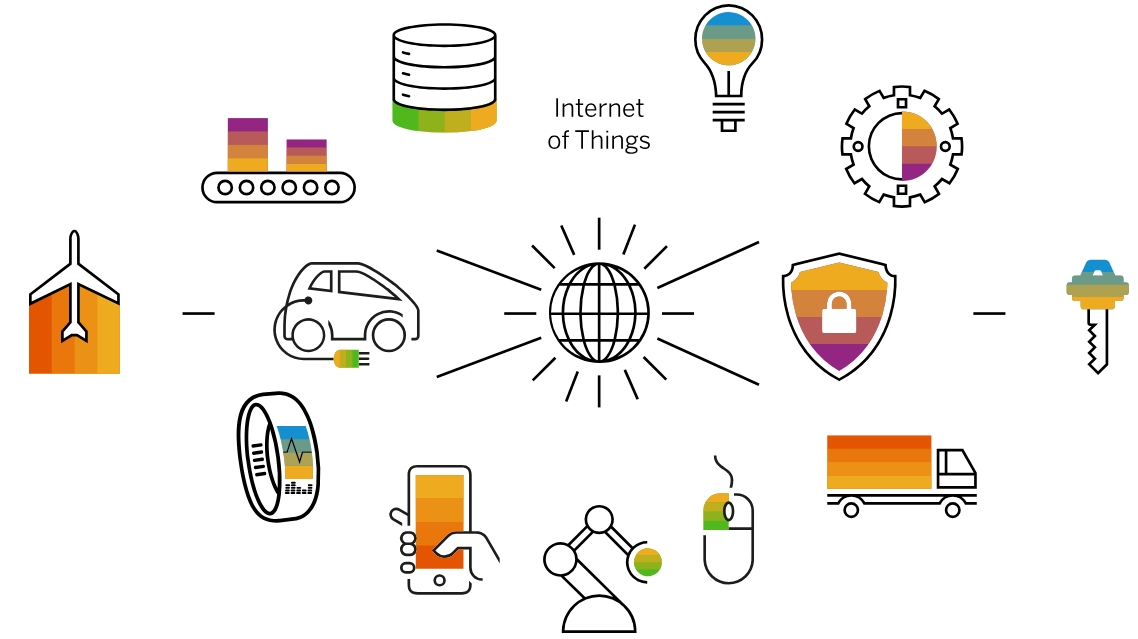
\includegraphics[width=1\linewidth]{imagenes_articulos/sp47_02} \end{center}
\figcaption{IoT. Fuente: https://goo.su/MEg6ePW}

\end{minipage}
\end {flushleft}

\textbf{Aporte del Cloud Computing a los sistemas de procesamiento integrado}

La computación en la nube ha revolucionado la gestión de los sistemas de procesamiento integrado (SPI) al ofrecer una infraestructura flexible, escalable y accesible.

Una ventaja clave es la escalabilidad, ya que los SPI en la nube pueden ajustar dinámicamente sus recursos según las necesidades, sin requerir grandes inversiones en hardware. Esto permite a las empresas adaptarse rápidamente a cambios en la demanda o nuevas oportunidades.

Además, la nube facilita el acceso a los SPI desde cualquier lugar, lo que mejora la colaboración entre equipos distribuidos y aumenta la eficiencia, especialmente en entornos de trabajo remoto.

\bigskip
\bigskip
\bigskip

\hypertarget{conclusiones-5}{%
\section{Conclusiones}\label{conclusiones-5}}

La integración de tecnologías emergentes como la IA, IOT y la computación en la nube en los Sistemas de Procesamiento Integrado (SPI) está revolucionando la gestión de recursos empresariales. La IA automatiza tareas repetitivas y proporciona análisis predictivos, mejorando la toma de decisiones y optimizando operaciones. El IoT permite el monitoreo en tiempo real y el mantenimiento predictivo, reduciendo costos y minimizando el tiempo de inactividad. Por su parte, la computación en la nube, ofrece escalabilidad, flexibilidad y accesibilidad, permitiendo a las empresas adaptarse rápidamente a las demandas del mercado y fomentar la colaboración en un entorno global. En conjunto, estas tecnologías no solo fortalecen la eficiencia operativa, sino que también posicionan a las empresas para un crecimiento sostenible en un entorno empresarial cada vez más dinámico.

\hypertarget{referencias-4}{%
\section{Referencias}\label{referencias-4}}

\begin{itemize}
\item
  {[}1{]} Erl, Thomas, Zaigham Mahmood, y Ricardo Puttini. Cloud Computing: Concepts, Technology \& Architecture. Upper Saddle River: Prentice Hall, 2020.
\item
  {[}2{]} Klaus Schwab, ``The Fourth Industrial Revolu-
  tion'', World Economic Forum, Fecha de consulta: 30 de julio 2024
  \href{https://www.weforum.org/about/the-fourth-industrial-revolution-by-klaus-schwab/}{https://www.weforum.org}
\item
  {[}3{]} Miller, Michael. The Internet of Things: How Smart TVs, Smart Cars, Smart Homes, and Smart Cities Are Changing the World. Indianapolis: Que Publishing, 2015.
\end{itemize}

\end {multicols}

\medskip

\HRule

\medskip

\hypertarget{pareja08}{%
\chapter{Evolución de las pruebas unitarias y de integración en la era DevOps}\label{pareja08}}

\begin{center}
\includegraphics[width=1\linewidth]{autores/pareja08_01} \end{center}

\begin {multicols}{2}

\textbf{\emph{Palabras clave:}} Testing, componentes, DevOps, calidad, CI/CD, requerimientos.

\hypertarget{introducciuxf3n-6}{%
\section{Introducción}\label{introducciuxf3n-6}}

La era DevOps es ahora, vivimos en mundo tecnológico que está cada vez más necesitado de software para uso personal, profesional y de servicios, la alta demanda de proyectos de software ha logrado que las prácticas de DevOps sean necesarias para la entrega contínua y eficiente, haciendo la fase de pruebas una de las más importantes para asegurar la calidad del producto que se entrega.

A continuación haremos un pequeño recorrido histórico desde el nacimiento de las pruebas unitarias y de integración hasta su participación en el esquema DevOps, para resaltar su importancia en el ciclo de desarrollo del software para entregar productos que cumplan los estándares de calidad y con los requerimientos funcionales solicitados.

\hypertarget{artuxedculo-6}{%
\section{Artículo}\label{artuxedculo-6}}

\textbf{Pruebas unitarias}

Las pruebas unitarias toman la unidad de código funcional más pequeña para realizar pruebas, con el objetivo de validar que cada una cumpla con su funcionalidad y propósito, detectar errores en etapas tempranas, documentar fácilmente el código y ayudar a mantener el estándar de calidad esperado, además de facilitar una futura integración contínua (CI).

\textbf{Pruebas de integración}

Las pruebas de integración garantizan que cada uno de las unidades de código del software funcionen en conjunto, que interactúen y se comuniquen como es esperado. Con las pruebas de integración es posible validar el correcto flujo de datos y el cumplimento de requerimientos funcionales. Las pruebas de integración están asociadas a la entrega contínua
(CD).

\bigskip
\bigskip
\bigskip

\textbf{CI/CD}

\emph{CI/CD se refiere a integración continua (CI) y entrega continua (CD), optimiza la integración del trabajo de múltiples desarrolladores en un solo producto de manera eficiente y precisa. En el contexto de DevOps, CI/CD acelera los procesos de codificación, pruebas e implementación al proporcionar un repositorio centralizado para el trabajo y herramientas de automatización} (IBM n.d.)

\textbf{DevOps}

DevOps combina el desarrollo (Dev) y las operaciones (Ops) para aumentar la eficiencia, la velocidad y la seguridad del desarrollo, integración y entrega de software. Las prácticas de DevOps permiten a los equipos de desarrollo de software y operaciones acelerar la entrega a través de la automatización, la colaboración, la retroalimentación rápida y la mejora iterativa. Las pruebas unitarias y de integración son una parte importante del ciclo DevOps de manera que, el código sea considerado listo para desplegarse después de superar las pruebas unitarias, y automáticamente desplegado después de pasar correctamente las pruebas de integración.

\begin {flushleft}
\noindent\begin{minipage}[c]{\columnwidth}

\begin{center}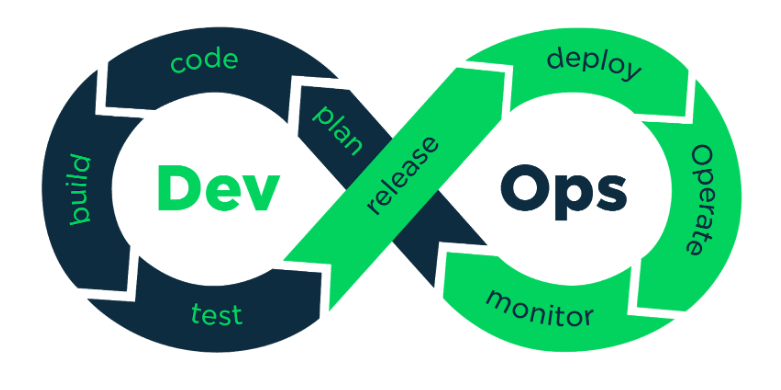
\includegraphics[width=1\linewidth]{imagenes_articulos/sp08_01} \end{center}
\figcaption{Esquema de DevOps. Fuente: https://acortar.link/6nG2Fj}

\end{minipage}
\end {flushleft}

\textbf{Evolución de las pruebas en la era DevOps}

La era DevOps nos ha traído un cambio de paradigma sobre la manera en la que se desarrolla y se despliega el software donde uno de los pilares fundamentales es la automatización, utilizando estos enfoques podremos acelerar el ciclo de desarrollo y asegurar la entrega confiable de software de alta calidad, siempre y cuando el proyecto esté bien definido. Esto ha impactado a los ambientes de pruebas, dándoles dentro del ciclo de vida del software un rol más importante, un rol que podríamos llamar el amigo odioso que suele señalar nuestros errores, pero sin él no sabemos cuáles aspectos podemos mejorar.

\begin {flushleft}
\noindent\begin{minipage}[c]{\columnwidth}

\begin{center}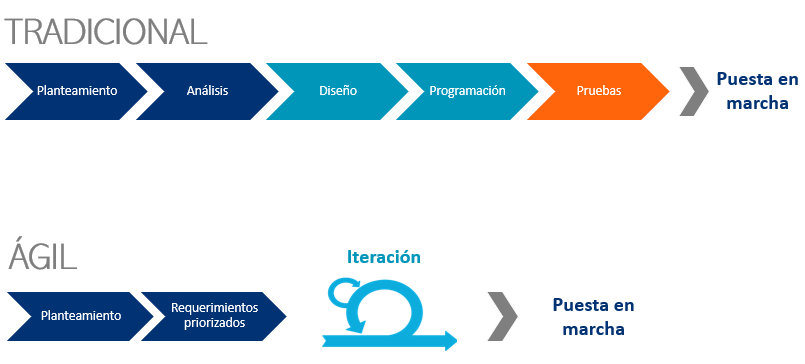
\includegraphics[width=1\linewidth]{imagenes_articulos/sp08_02} \end{center}
\figcaption{Esquema comparativo, Tradicional vs Ágil. Fuente: https://acortar.link/87ogc8}

\end{minipage}
\end {flushleft}

Antes de DevOps, las pruebas se realizaban al final del ciclo; ahora, con DevOps, se integran desde el inicio, mejorando la eficiencia y calidad, y así evitamos problemas con nuestro product manager. Entre algunos Frameworks de pruebas de este tipo podemos encontrar ejemplos como Junit o Jest, estos nos proporcionan un entorno para escribir y ejecutar pruebas unitarias de una manera estructurada, en nuestra opinión, Jest es un framework bastante amigable.

Con las metodologías de desarrollo tradicionales el proceso solía ser más lineal y en nuestra opinión muy lento, esto era una desventaja debido a que el software podría tener fallas complejas de solucionar y nos exponíamos a tener que solucionarlas en una etapa muy avanzada del proyecto; utilizando DevOps las pruebas de integración se ejecutan posterior a las pruebas unitarias en fases tempranas, las cuales son encargadas de verificar que el sistema y sus componentes cumplan con sus funcionalidades.

\bigskip
\bigskip
\bigskip

\hypertarget{conclusiones-6}{%
\section{Conclusiones}\label{conclusiones-6}}

Las pruebas unitarias y de integración en la era DevOps han transformando el ciclo del desarrollo de software a lo largo del tiempo, proporcionándonos un marco ágil y eficiente que asegura la calidad y la funcionalidad de nuestro producto final. Seguir una cultura DevOps resalta la importancia de integrar las pruebas para que así, podamos utilizarlas en fases tempranas del desarrollo. Durante el desarrollo antes de la era DevOps, las pruebas se
ejecutaban de manera aislada y tardía, lo que afectaba al proyecto detectando errores en fases avanzadas del desarrollo, restando a la calidad de los entregables y represando un obstáculo al cumplimiento de los requerimientos funcionales y no funcionales. Por lo tanto, es recomendable adoptar una cultura DevOps que ejecute pruebas desde las primeras fases de desarrollo para garantizar una entrega continua y un producto de alta calidad.

\hypertarget{referencias-5}{%
\section{Referencias}\label{referencias-5}}

\begin{itemize}
\item
  {[}1{]} MTP Internacional. ``Pruebas de Software en la era DevOps, Integración Continua y Entrega Confiable.'' Última modificación julio 7, 2023.
  \href{https://mtpinternational.mx/testing-de-software/pruebas-de-software-en-la-era-devops-integracion-continua-y-entrega-confiable/}{https://mtpinternational.mx}
\item
  {[}2{]} ¿Qué son las pruebas de software? (2024, mayo 14). Ibm.com. \href{https://www.ibm.com/es-es/topics/software-testing}{https://www.ibm.com}
\item
  {[}3{]} ``¿Qué son las pruebas unitarias?''. AWS. Recuperado el 3 de agosto de 2024, de \href{https://aws.amazon.com/es/what-is/unit-testing/}{https://aws.
  amazon.com}
\item
  {[}4{]} TRBL Services. ``Introducción a DevOps. Qué es y cómo implementarlo.'' Marzo 24, 2021. \href{https://trbl-services.eu/blog-introduccion-devops/}{https://trbl-services.eu}
\item
  {[}5{]} What is DevOps? (2022, febrero 10). Gitlab.com; GitLab. \url{https://about.gitlab.com/topics/devops/}
\end{itemize}

\end {multicols}

\medskip

\HRule

\medskip
%%%%%% SECCION 3
\includepdf{images/seccion3.pdf}

\AddEverypageHook{%
\ifthenelse{\value{page}<37}%
{\ifthenelse{\isodd{\value{page}}}%
  	{\backgroundsetup{scale=1, color=white, opacity=1, angle=0, contents={
\includegraphics[width=\paperwidth,height=\paperheight]{latex/background_numberimpar.pdf}}}}%
  	{\backgroundsetup{scale=1, color=white, opacity=1, angle=0, contents={
\includegraphics[width=\paperwidth,height=\paperheight]{latex/background_numberpar.pdf}}}}%
}{}%
\BgMaterial}
%%%%%%%%%%%%%%%%%%%%%%%%%%%

\hypertarget{victor}{%
\chapter{Aplicaciones reactivas y el aumento de la complejidad en el desarrollo de software}\label{victor}}

\begin{center}
\includegraphics[width=1\linewidth]{autores/pareja00_victor} \end{center}

\begin {multicols}{2}

\textbf{\emph{YouTube:}} \url{https://youtu.be/hsWrSGepTdA}

\hypertarget{entrevista-2}{%
\section{Entrevista}\label{entrevista-2}}

\textbf{¿Quién es el Ing. Víctor Orozco y cuál es su experiencia relevante en el ámbito de la tecnología?}

Me defino como un obrero del código con 15 años de experiencia como desarrollador de software. Actualmente, en Nabenik, trabajo como profesor universitario y consultor para sectores como banca, telecomunicaciones y gobierno. Me enfoco en arquitectura de software, buenas prácticas de desarrollo y capacitación de equipos. Además, participo en los programas Java Champions y Oracle, que fomentan comunidades de desarrolladores y buenas prácticas a nivel global.

\textbf{¿Qué es Nabenik y qué papel desempeña en el sector tecnológico?}

Fundamos la empresa como una consultoría de software. Después de que estuve en el extranjero de 2012 a 2014, regresé a Guatemala y junto a mi socio, Luis Pedro Estrada, expandimos el negocio para incluir tercerización de recursos, capacitaciones y representación de productos, siempre alineados con la demanda del mercado. Nabenik, que significa \emph{``conocimiento''} y \emph{``viento''} en mam, se enfoca principalmente en el mercado centroamericano, aunque también hemos trabajado en México, Latinoamérica, Estados Unidos y España. Nos definimos como una consultoría de software que acompaña todo el proceso de transformación digital.

\textbf{¿Cuál fue su principal motivación para crear Nabenik? ¿Qué desafíos significativos enfrentó y cómo los superó?}

Mi motivación para emprender en Guatemala fue accidental, surgió al desarrollar una aplicación móvil en un contexto donde había poco desarrollo en ese ámbito. Esto llevó a la necesidad de formalizar la empresa por razones fiscales y de facturación, permitiéndonos crecer y delegar funciones. Sin embargo, enfrentamos dificultades, como la falta de acceso a capital de riesgo, lo que nos obligó a optar por un periodo de bootstrap para reinvertir las ganancias. Aprendí que un negocio solo es viable si satisface necesidades reales y genera ingresos, lo cual fue un reto, especialmente por mi perfil técnico, lo que me llevó a aprender sobre la marcha.

\textbf{¿Qué son las aplicaciones reactivas y cuáles son sus características distintivas?}

Las aplicaciones reactivas surgen de la demanda actual de usuarios que esperan experiencias fluidas y eficientes. A diferencia de principios de los 2000, hoy las aplicaciones están diseñadas para un público amplio, enfrentando retos técnicos para manejar miles de usuarios. El Reactive Manifesto establece cuatro características esenciales: deben ser responsivas, elásticas (capaces de escalar con la demanda), resilientes (recuperarse automáticamente de fallos) y tener un enfoque de mensajería, donde las aplicaciones funcionan como un conjunto de pequeños servicios en lugar de un monolito. En resumen, las aplicaciones reactivas son una forma de construir sistemas distribuidos que optimizan recursos y costos para soportar un alto número de usuarios.

\textbf{¿Cómo se diferencia el modelo de programación reactiva del modelo de programación de enfoque imperativo?}

Es importante distinguir entre una aplicación reactiva y un lenguaje de programación con patrones reactivos; la primera se centra en la arquitectura, mientras que el segundo aborda cómo se genera el código. Tradicionalmente, lenguajes como Java y .NET utilizaban un modelo de programación blocking, donde pocos hilos atendían múltiples clientes, lo que podía causar cuellos de botella. La solución, popularizada por Node.js, fue adoptar paradigmas de programación reactivos, donde un solo hilo gestiona eventos en un bucle, permitiendo procesar múltiples solicitudes sin bloquear el sistema. Aunque esto resuelve muchos problemas de concurrencia, su complejidad requiere programadores capacitados, a diferencia de la programación imperativa.

\bigskip
\bigskip
\bigskip
\bigskip
\bigskip
\bigskip

\textbf{¿Qué estrategias recomienda para gestionar la complejidad del código en aplicaciones reactivas?}

Recomiendo dos estrategias para manejar la programación reactiva: primero, aprovechar las características de lenguajes como Kotlin y JavaScript, que ofrecen estructuras para gestionar callbacks eficientemente, como las corrutinas en Kotlin y async/await en JavaScript. La segunda estrategia es utilizar patrones de tipo RX, comunes en Angular y RX Java, que permiten ejecutar tareas en cola y encadenar funciones de manera reactiva. En cuanto a tendencias, creo que los hilos tradicionales quedarán en desuso, siendo reemplazados por virtual threads en nuevas versiones de la máquina virtual de Java, lo que permitirá una ejecución más eficiente del código imperativo. Las tres formas principales de implementar programación reactiva son: aprovechar las facilidades de los lenguajes, usar bibliotecas reactivas como RX y adoptar virtual threads.

\textbf{¿Cómo influye la programación reactiva en la depuración y el manejo de errores dentro de una aplicación?}

El mayor reto de la programación reactiva es la depuración, especialmente al trabajar con callbacks, ya que el flujo de ejecución es asíncrono y salta de una función a otra, dificultando la identificación de errores. En JavaScript, aunque las funciones son ciudadanos de primer nivel, es complicado rastrear fallos. En Java o C\#, donde se utilizan expresiones lambda, los stack traces se vuelven más detallados, haciendo aún más difícil localizar el problema. Aunque herramientas como async/await o corrutinas pueden ayudar, depurar código reactivo sigue siendo más complejo que en la programación imperativa, debido a la falta de una secuencia clara de ejecución.

\textbf{¿Cuáles son las mejores prácticas para gestionar estados y eventos en aplicaciones reactivas?}

En aplicaciones pequeñas, la gestión suele hacerse a través de bibliotecas, pero en aplicaciones distribuidas grandes se introduce un bus de comunicación y patrones más complejos. Dos patrones comunes son el event sourcing, donde se registran eventos en un bus (como Kafka) para que sean consumidos por otros componentes, y CQRS, que separa las operaciones de lectura y escritura. En CQRS, los comandos alteran el estado sin requerir una respuesta inmediata, mientras que las consultas notifican al usuario sobre la finalización de esos comandos. Para implementar programación reactiva a gran escala, es crucial dominar la comunicación de eventos, utilizando herramientas como Kafka, Camel, o servicios en la nube como SQS o SNS. Es fundamental entender que se está programando actores (microservicios) que responden a eventos en lugar de seguir un enfoque imperativo tradicional.

\textbf{¿Qué consideraciones deben tenerse en cuenta al definir requisitos y entregables en proyectos que utilizan programación reactiva y enfoques similares?}

Es fundamental evaluar si realmente se necesita programación reactiva. Aunque se puede implementar un sistema reactivo con programación imperativa, no siempre es necesario. En sistemas con pocos usuarios (100 a 500), seguir con un enfoque blocking tradicional es más práctico y ha funcionado durante años. Incluso empresas como Netflix, que utilizan Java y Spring, prefieren el código imperativo por su simplicidad en la depuración y la observabilidad, a pesar de tener arquitecturas distribuidas.

En contextos donde se justifica, como la ingesta de datos, frameworks reactivos como Vert.x o Spring Reactor pueden ser útiles. Sin embargo, en sistemas simples, la programación reactiva puede complicar más que ayudar. Un buen arquitecto debe evaluar si la programación reactiva realmente aporta valor y, si es así, determinar qué partes del sistema deben ser reactivas y cuáles pueden seguir siendo síncronas, creando una arquitectura equilibrada.

\textbf{¿Qué bibliotecas o frameworks son populares para el desarrollo de aplicaciones reactivas y cómo simplifican el proceso, dado su potencial para aumentar la complejidad?}

En la actualidad, en el contexto de la JVM, las corrutinas son muy populares en Kotlin, mientras que para Java, Spring WebFlux, basado en Spring Reactor, es el framework más utilizado. Vert.x también es relevante, especialmente por su respaldo de RedHat y sus múltiples abstracciones, aunque programar a bajo nivel con Vert.x puede parecerse al uso de callbacks. Es importante considerar que las bases de datos deben contar con drivers reactivos compatibles.

La JVM ofrece APIs como Completable Futures para la programación reactiva sin necesidad de frameworks específicos. Si el backend es Java y el frontend es TypeScript, se recomienda explorar RX para mantener un paradigma de programación coherente entre ambos. Además, dominar async/await en TypeScript y JavaScript es fundamental, ya que es una herramienta clave para la mayoría de los programadores antes de abordar patrones más complejos que justificarían el uso de RX.

\bigskip
\bigskip
\bigskip

\textbf{¿Cómo se integra la programación concurrente y distribuida en el diseño de aplicaciones reactivas?}

La programación concurrente y la programación reactiva son conceptos complementarios. La concu-
rrencia se refiere a la ejecución de hilos y su coordinación, a menudo enseñada a través de semáforos y modelos de concurrencia. En contraste, la programación reactiva abstrae estos conceptos, permitiendo que los programadores se centren en el envío de eventos a un bucle de procesamiento sin preocuparse por los hilos subyacentes.

Node.js, por ejemplo, utiliza un event loop y puede manejar múltiples hilos para diversas tareas. La programación reactiva se basa en esta concurrencia para funcionar eficazmente. Aunque la programación distribuida y la reactiva suelen estar relacionadas, no son condiciones mutuamente exclusivas; se puede crear una aplicación monolítica con APIs reactivas o una aplicación distribuida con código imperativo. La elección de usar uno u otro dependerá de las necesidades específicas del proyecto.

\textbf{¿Cuáles son las principales dificultades en el mantenimiento de aplicaciones reactivas en comparación con aplicaciones tradicionales?}

El seguimiento del código en aplicaciones legacy, que suelen tener muchos años de éxito, plantea desafíos significativos, especialmente en su manteni-
miento. A menudo, los desarrolladores se enfocan en lanzar aplicaciones rápidamente sin considerar su sostenibilidad a largo plazo. Para mitigar problemas futuros, se recomienda usar lenguajes de programa-
ción tipados, como TypeScript, que facilitan la lectura y comprensión del código. A medida que los proyectos envejecen, la falta de tipado en lenguajes como JavaScript puede dificultar la comprensión del código original, que puede estar lleno de diversas estructuras. La clave es optar por lenguajes que promuevan un tipado explícito para mejorar la mantenibilidad y evitar que el código se convierta en ``código espagueti''.

\textbf{¿Se puede simplificar el mantenimiento de aplicaciones reactivas complejas sin comprometer la funcionalidad o el rendimiento?}

La complejidad en el código a menudo surge del uso de callbacks. Se recomienda migrar a async/await si se utilizan callbacks explícitos, y adoptar sistemas de tipos cuando sea posible. Si un lenguaje ofrece opciones como corrutinas (por ejemplo, en Go), es preferible utilizarlas. Los lenguajes evolucionan constantemente; por ejemplo, los virtual threads en Java son una característica reciente. Mantenerse actualizado con las mejoras del lenguaje es crucial para facilitar el mantenimiento de aplicaciones y gestionar la deuda técnica. Es importante destinar tiempo en los proyectos para abordar esta deuda y evitar su acumulación.

\textbf{Mensaje final para quienes estén interesados en el desarrollo de aplicaciones reactivas y tecnológicas avanzadas}

Entre 2000 y 2010, tras la \emph{burbuja punto-com}, Java y .NET dominaron como plataformas generales, aunque PHP y otras herramientas de software libre también ganaron popularidad. Sin embargo, con el avance de la tecnología y el uso de smartphones, este enfoque ha cambiado, y ya no existen plataformas únicas.

Los desarrolladores modernos deben ir más allá de simplemente aprender a programar. Es fundamental dominar patrones de diseño, patrones de programación y herramientas para gestionar sistemas distribuidos y arquitecturas, como la programación serverless, microservicios en Kubernetes e infraestruc-
tura como código.

El panorama actual es mucho más complejo que hace una década. Por ello, se recomienda especializarse en una tecnología, pero también adquirir conocimientos sobre arquitectura y mantener-
se actualizado con las tendencias y soluciones en la ingeniería de software.

\end {multicols}

\medskip

\HRule

\medskip

\hypertarget{pareja11}{%
\chapter{Facilitar la gestión de proyectos de software desde el uso de herramientas digitales}\label{pareja11}}

\begin{center}
\includegraphics[width=1\linewidth]{autores/pareja11_01} \end{center}

\begin {multicols}{2}

\textbf{\emph{Palabras clave:}} Proyectos, Gestión, Software, Recursos, Productividad, Adaptación.

\hypertarget{introducciuxf3n-7}{%
\section{Introducción}\label{introducciuxf3n-7}}

La evolución de la gestión de proyectos de software ha recorrido un largo viaje que ha sido capaz de reflejar como ha progresado la tecnología y cómo cubre las necesidades cambiantes del ser humano. Destaca la crisis del software como ese disparador para la creación e implementación de herramientas especializadas para ofrecer soluciones adaptadas -- sirviendo como facilitadores para una gestión efectiva en el desarrollo del software.

Hoy en día con los cambios constantes en los avances de la tecnología digital, la gestión de proyectos de software no se queda atrás ya que muchos de los procesos que eran manuales pasaron a ser automatizados, optimizados y gestionan de mejor manera contando con distintas opciones, siempre y cuando se adapten a las necesidades del negocio, equipo de
trabajo y proyecto que se esté realizando.

\hypertarget{artuxedculo-7}{%
\section{Artículo}\label{artuxedculo-7}}

\textbf{La evolución de la gestión de proyectos de software -- desde sus inicios hasta hoy}

La humanidad, desde tiempos inmemorables, ha realizado diferentes tipos de proyectos. No se le atribuye la gestión de proyectos a nadie, pero cabe destacar que, en los diferentes entornos como la industria, la ciencia o el arte, se ha utilizado esta gestión, por lo que las técnicas desarrolladas han ido evolucionado junto con estas. En el ámbito del software, se dan sus primeros pasos desde finales de los años 60s e inicio de los 70s con el auge de las computadoras y la metodología Ad Hoc -- improvisada además de que no seguía un plan específico. Dado como resultado la primera crisis del software.

Con la complejidad creciente de los sistemas informáticos, se evidenció la necesidad de la implementación de una formalidad -- naciendo así la gestión de proyectos de software: herramientas y prácticas para manejar con enfoques más efectivos además de eficientes, las nuevas exigencias que el software produce.

\textbf{Herramientas destacadas para impulsar y respaldar la gestión de proyectos de software en la actualidad}

\begin {flushleft}
\noindent\begin{minipage}[c]{\columnwidth}

\begin{center}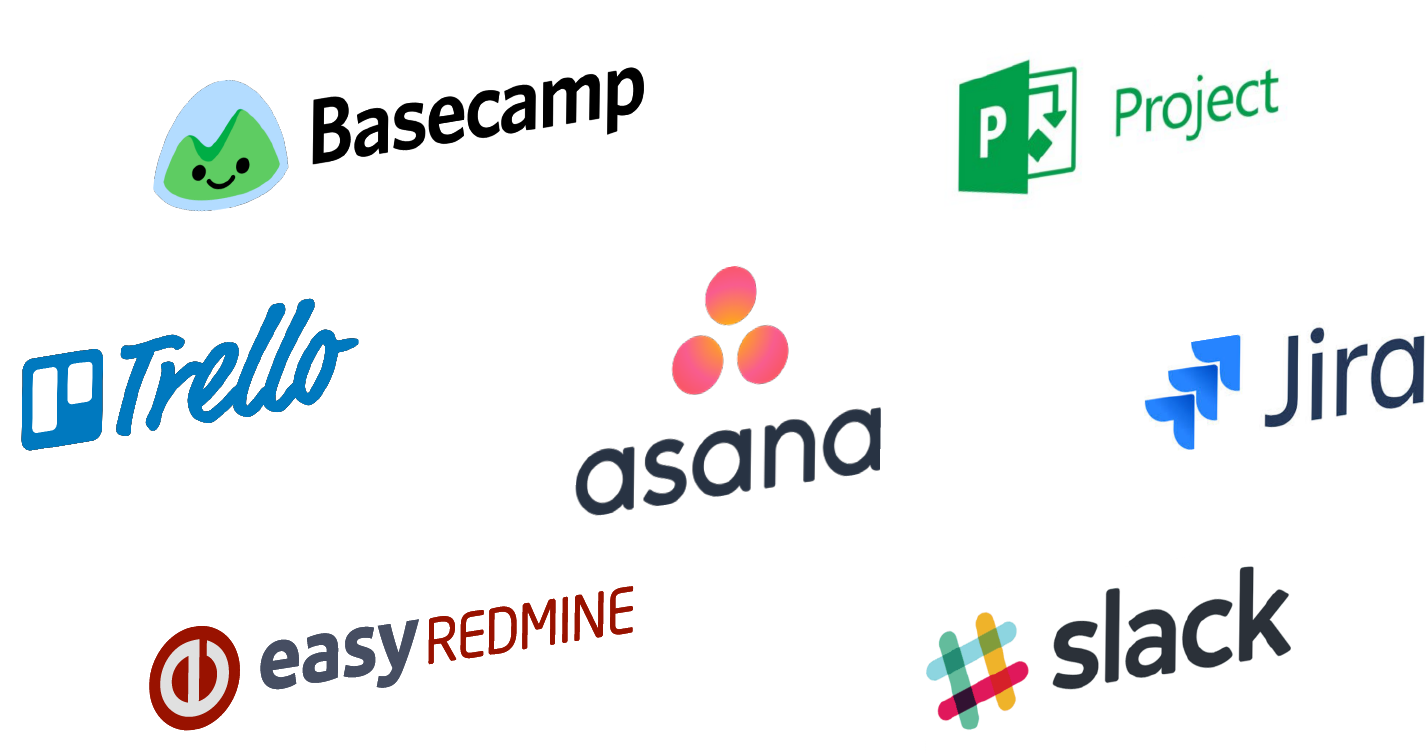
\includegraphics[width=0.9\linewidth]{imagenes_articulos/sp11_01} \end{center}
\figcaption{Herramientas de gestión de proyectos de software.}

\end{minipage}

\end {flushleft}

Destacan actualmente aquellas herramientas que facilitan la administración de los procesos de software. Dependerá del objetivo final de cada empresa o individuo su elección de herramienta, pero actualmente, se pueden mencionar herramientas como principales competidores Jira, Asana o Trello. Siendo el primero, una solución para el desarrollo de
software y trabajo en equipo. El segundo, ofreciendo ser una solución completa integrando el desarrollo de software y gestión de trabajo, útil para aquellas empresas dinámicas. El último, siendo útil para la gestión de proyectos pequeños.

Hoy en día es muy significativo usar herramientas de gestión de proyectos, pero se tienen que tomar en cuenta ciertos factores como las necesidades o los desafíos del proyecto evaluando cuál software es cubre esa necesidad, también puede enlistar las distintas aplicaciones que pueden dar un impacto al proyecto. Si ya se cuenta con una lista de posibles aplicaciones, es necesario probarlas con el equipo de trabajo para recibir una retroalimentación de este para utilizar la retroalimentación para poder adaptar el software al proyecto. Finalmente, es importante realizar un análisis de costos para justificar la elección siempre considerando los recursos disponibles.

Al contar con herramientas de software que se adapten a tu negocio, así como a tu proyecto, llega a tener un impacto significativo como el aumento de la productividad, la optimización de recursos, la mejora de tanto la comunicación como la colaboración, una mejor gestión de riesgos, mayor la transparencia y responsabilidad. Por último, también facilita la generación de reportes en tomar decisiones. Muchos de estos cambios se deben a que los procesos manuales que eran a papel y lápiz se pasaron a tecnologías para una mejor gestión de proyectos.

\hypertarget{conclusiones-7}{%
\section{Conclusiones}\label{conclusiones-7}}

La evolución de la gestión de proyectos de software es una gran evidencia del progreso que ha tenido la tecnología al ser utilizada para utilizarse como herramienta que se adapta y satisface a las necesidades cambiantes de la humanidad. Desde acontecimientos como la crisis del software, hasta la automatización de procesos manuales, la gestión de proyectos ha evolucionado considerablemente. Hoy en día, herramientas como Jira, Asana o Trello, por mencionar algunas, han transformado la manera en la que personas y empresas gestionan el software, que puede notarse en la mayor eficiencia y optimización de recursos que permiten una mejor colaboración y toma de decisiones. Es esencial que empresas e individuos seleccionen aquellas herramientas que mejor se adaptan a su proyecto -- parte clave para el
éxito en la gestión en el desarrollo de software.

\hypertarget{referencias-6}{%
\section{Referencias}\label{referencias-6}}

\begin{itemize}
\item
  {[}1{]} Casallas, Rubby.``¿Aún en Crisis? Algunos Mitos y desafíos de la Ingeniería de Software''. En Revista Sistemas No.~102 -- ACIS. Octubre - Diciembre 2007. Acceso el 26 de julio del 2024. \href{https://acis.org.co/portal/Revista/102/columnista.pdf}{https://acis.org.co}
\item
  {[}2{]} Cawley, Conor. ``6 Ways Technology Has Changed Project Management''. Tech.co. 10 de Mayo de 2023. Acceso el 3 de mayo de 2024. \href{https://tech.co/project-managementsoftware/ways-technology-has-changed-project-management}{https://tech.co}
\item
  {[}3{]} Raeburn, Alicia. ``Los 12 mejores software de gestión de proyectos en 2024''. Asana. 16 de febrero de 2024. Acceso el 26 de julio del 2024. \href{https://asana.com/es/resources/best-project-management-software}{https://asana.com}
\item
  {[}4{]} Virtual Space. ``7 Important Criteria for Project Management Tools''. 18 de Noviembre de 2022. Acceso el 3 de agosto de 2024. \href{https://virtualspace.ai/blogs/7-important-criteria-for-project-management-tools}{https://virtualspace.ai}
\item
  {[}5{]} Virtual Space. ``The Importance of Project Management Tools for Your Business''. 13 de Junio de 2023. Acceso el 3 de agosto de 2024. \href{https://virtualspace.ai/blogs/the-importance-of-project-management-tools-for-your-business}{https://virtualspace.ai}
\item
  {[}6{]} Wallace, William. (2014). ``Gestión de Proyectos''. Edinburgh Business School (EBS) -- Heriot-Watt University. Acceso el 26 de julio del 2024. \href{https://ebs.online.hw.ac.uk/documents/course-tasters/spanish/pdf/pr-bk-taster.pdf}{https://ebs.online.hw.ac.uk}
\end{itemize}

\end {multicols}

\medskip

\HRule

\medskip

\hypertarget{pareja33}{%
\chapter{Maximización en la ingeniería de requerimientos con inteligencia artificial}\label{pareja33}}

\begin{center}
\includegraphics[width=1\linewidth]{autores/pareja33_01} \end{center}

\begin {multicols}{2}

\textbf{\emph{Palabras clave:}} Software de Requerimientos, Ingeniería de Requerimientos, Inteligencia Artificial, Ambigüedad, Maximizar, Calidad.

\hypertarget{introducciuxf3n-8}{%
\section{Introducción}\label{introducciuxf3n-8}}

Conforme los años pasan, la globalización y tecnologías mejoran. El uso indispensable de sistemas y el desarrollo de proyectos de alta calidad se vuelven más exigentes y complejos. La ingeniería de requerimientos juega un papel fundamental, siendo la base de cualquier proyecto y su mala planificación y desarrollo puede determinar si un proyecto va a fracasar.

La inteligencia artificial y más específicamente el procesamiento del lenguaje natural, llega a ser una herramienta poderosa que puede ser de gran ayuda para el análisis de todas las fases de la ingeniería de requerimiento, implementando mejoras específicas para maximizar la calidad de la toma de requerimientos y por consiguiente mejores bases para la construcción de cualquier proyecto.

\hypertarget{artuxedculo-8}{%
\section{Artículo}\label{artuxedculo-8}}

\textbf{Ingeniería de requerimientos}

¿Alguna vez te has preguntado cómo un proyecto puede triunfar o fracasar? Esto obviamente viene ligado a varios factores, como el utilizar una tecnología inadecuada, pruebas insuficientes, problemas con la gestión de recursos, entre otros. Pero, lo que va a decidir si un proyecto va a triunfar o fracasar será el cómo se construyen sus bases, por lo cual la ingeniería de requisitos es considerada como la fase más importante en los proyectos de software.

La ingeniería de requerimientos se describe como la disciplina que abarca los procesos para especificar los requisitos, analizarlos y perfeccionarlos para el comienzo de su desarrollo. Esta presenta diferentes fases que comienzan con la de elicitación, que es la manera de extraer información importante de alguien a través de una conversación educada o cotidiana. Siendo esta la que declara los requerimientos para especificación y propósito del software, siguiendo con la fase de análisis, donde a los requerimientos se deben analizar para que cumplan con una
buena consistencia y exactitud, luego sigue la fase de documentación, en la cual se negocian y verifican los requerimientos con los stakeholders, personas interesadas, y por último la fase de gestión, donde se hacen los cambios respectivos a los requerimientos.

\textbf{Desafíos en la búsqueda de los requerimientos }

A lo largo del tiempo, las fases de la ingeniería de requerimientos pasaron a ser lineales a ser iterativas, esto a causa de cambios en el entorno del cliente o de errores en el análisis de todo el proceso. La ingeniería de software no es invulnerable a actividades poco eficientes en cada una de las fases que la conforman, ocasionando problemas que afecten directamente al desarrollo del software.

De esto llegan a surgir requisitos ambiguos, estos siendo definidos de forma vaga por errores de comunicación por ambas partes del proyecto, que a la larga van a afectar con el desarrollo de este. También hay otros factores a considerar como la baja participación de todos los comprometidos en la elaboración de los requisitos, dando lugar a requisitos conflictivos que no cuentan con la precisión necesaria. Todo esto afecta directamente la trazabilidad, siendo este el
proceso que define cada uno de los requerimientos desde su concepción hasta su implementación en el código fuente.

\textbf{Inteligencia artificial}

Hoy en día la inteligencia artificial juega un papel muy importante en todo el mundo, llegando a transformar algunos aspectos cotidianos hoy en día, pero generando un gran impacto en el mundo de la tecnología.

Está definiéndose como las máquinas tienen la capacidad de aprender a través de diferentes experiencias, con el fin de acercarse a lo más cercano del comportamiento humano. Actualmente, la inteligencia artificial se encarga de la automatización de procesos, los algoritmos de búsqueda, el procesa-
miento de lenguaje natural, la automatización de procesos, el reconocimiento de patrones, la conducción automatizada, entre otros.

\textbf{La unión hace la fuerza}

A lo largo de los años han surgido investigaciones de como la capacidad de la inteligencia artificial podría repercutir en la ingeniería de requerimientos, con el fin de mejorar la calidad del software entregado, el tiempo de desarrollo y obviamente brindando un gran apoyo a los profesionales. Esto utilizando técnicas para optimizar cada una de las fases del ciclo del desarrollo del software, como la mejora de la coordinación entre ambas partes, incluyendo la mejora de comunicación para evitar conflictos a futuro; todo esto priorizando la trazabilidad de los requisitos, teniendo como resultado el máximo rendimiento. A continuación, se presenta una tabla con los aportes de la IA a cada una de las fases de la ingeniería de requerimientos:

\begin {flushleft}
\noindent\begin{minipage}[c]{\columnwidth}

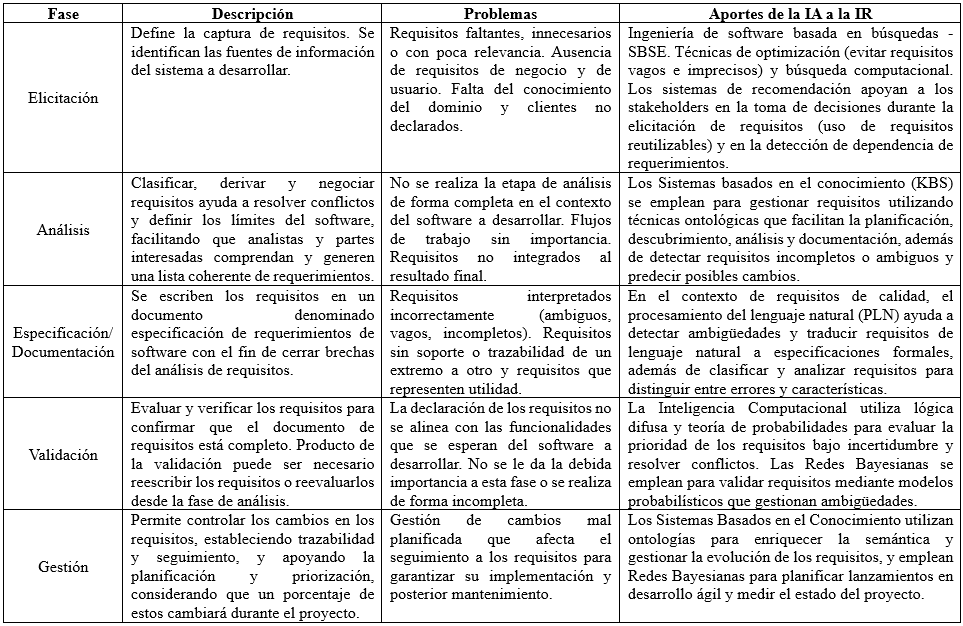
\includegraphics[width=1\linewidth]{imagenes_articulos/sp33_01}
\tabcaption{Fases de la ingeniería de requerimientos y técnicas de IA. Fuente: https://goo.su/v2R7h}

\end{minipage}
\end {flushleft}

Mediante el aprendizaje de los componentes semánticos de historias de usuarios, la IA sería capaz de proporcionar proyecciones del esfuerzo necesario para completar cada uno, esto facilitando la planificación de todo un proyecto de software, repercutiendo en una mejor producción. También está la idea de que se puede aplicar diferentes paradigmas para la reducción de errores y con ello la optimización de procesos, problemas que persisten hoy en día.

\bigskip
\bigskip
\bigskip

\textbf{El estigma del uso de IA}

A pesar de las grandes ventajas como herramienta que apoyo que ofrece la IA en la ingeniería de requerimientos, muchos profesionales aún son escépticos en el uso de esta, por diferentes motivos como, por ejemplo, la veracidad de los datos, temas más intrínsecos como el ego que puede llegar a sentir una persona cuando una herramienta de IA llega a realizar su \emph{``trabajo''} de mejor manera. Todos estos aspectos pueden provocar que la adopción de estas herramientas
para empresas, consultoras o ingenieros llegue a ser un poco más complicada.

\hypertarget{conclusiones-8}{%
\section{Conclusiones}\label{conclusiones-8}}

La ingeniería de requerimientos es sin duda la parte más fundamental y la columna vertebral de todo proyecto, de esta depende si un proyecto fracasará o no, vale la invertir recursos en todas las fases e iteraciones para lograr que los cimientos sean seguros para el completo desarrollo de la obra.

Con el auge de la IA, la ingeniería de requerimientos experimentará el punto más alto de calidad al momento del desarrollo de proyectos, ya que las iteraciones continuas y el constante asesoramiento de esta herramienta dará hincapié a la reducción de tiempos, minimización de errores y ambigüedades, claridad en todas las etapas y como resultado mejores sistemas.

\hypertarget{referencias-7}{%
\section{Referencias}\label{referencias-7}}

\begin{itemize}
\item
  {[}1{]} Sanguino-Reyes, Magreth Rossio, y Byron Cuesta-Quintero. 2022. «La Inteligencia Artificial En ``La ingeniería De Requerimientos: Un Estudio De Mapeo sistemático''. Mundo FESC 12 (23):209-24. \url{https://goo.su/v2R7h}
\item
  {[}2{]} Arenas Seleey, Daniel, Cristian Eduardo Prieto Triana, y Diana Carolina Chacón López. 2022. ``Ingeniería De Requerimientos E Inteligencia Artificial: Una revisión De La Literatura''. Revista Colombiana de Tecnologias de Avanzada (RCTA) 1 (39):100-106. \url{https://goo.su/vXJvz9}
\end{itemize}

\end {multicols}

\medskip

\HRule

\medskip

\hypertarget{pareja55}{%
\chapter{Futuro del Mantenimiento de Software: Cambiando las reglas con el Reinforcement Learning}\label{pareja55}}

\begin{center}
\includegraphics[width=1\linewidth]{autores/pareja55_01} \end{center}

\begin {multicols}{2}

\textbf{\emph{Palabras clave:}} Mantenimiento correctivo, Manteni-
miento preventivo, Mantenimiento adaptativo, Inteligencia artificial, Machine Learning, Deep Learning.

\hypertarget{introducciuxf3n-9}{%
\section{Introducción}\label{introducciuxf3n-9}}

La calidad y la fiabilidad del software son fundamen-
tales para el funcionamiento de nuestra sociedad moderna. Para garantizar que el software siga siendo relevante y útil, es necesario un mantenimiento continuo. Este proceso va más allá de la simple corrección de errores e implica adaptar las aplicaciones a nuevas tecnologías, mejorar su rendimiento y asegurar su compatibilidad con diversos sistemas.

El aprendizaje mediante refuerzo está empoderando al software para tomar decisiones de manera autónoma, optimizando su funcionamiento y mejoran-
do su capacidad para responder a las demandas de los usuarios. Al aprender de sus interacciones con el entorno, los sistemas basados en aprendizaje por refuerzo pueden identificar patrones, predecir fallos y tomar medidas correctivas de forma proactiva.

\hypertarget{artuxedculo-9}{%
\section{Artículo}\label{artuxedculo-9}}

En el dinámico mundo de la tecnología, el mantenimiento de software emerge como un pilar fundamental para asegurar la estabilidad y eficacia de las soluciones digitales. Este proceso, a menudo subestimado, no solo corrige errores y mejora la funcionalidad del software, sino que también juega un papel crucial en la adaptación a los constantes cambios del entorno tecnológico. El mantenimiento de software abarca un conjunto de actividades diseñadas para
preservar y optimizar un sistema tras su despliegue inicial. Se trata de modificar un sistema de software después de su entrega para corregir fallos, mejorar el rendimiento o adaptar el software a un entorno cambiante.

\bigskip
\bigskip
\bigskip
\bigskip
\bigskip
\bigskip

¿Por qué es vital el mantenimiento de software? La respuesta es simple, pero poderosa. Un software bien mantenido asegura la continuidad del servicio y minimiza las interrupciones, un factor crucial en un entorno donde la disponibilidad continua es esencial.

Además, la seguridad es una preocupación constante; el mantenimiento regular permite aplicar parches y actualizaciones para proteger contra vulnerabilidades emergentes. El Dr.~Ian Sommerville, autor destacado en ingeniería de software, enfatiza que \emph{``un programa usado en un entorno real debe cambiar; de otro modo, en dicho entorno se volvería progresivamente inútil''}. Este punto de vista subraya la importancia de una gestión proactiva del manteni-
miento.

\begin {flushleft}
\noindent\begin{minipage}[c]{\columnwidth}

\begin{center}
\includegraphics[width=0.8\linewidth]{imagenes_articulos/sp55_01} \end{center}
\figcaption{Portada del libro Software Engineering del Dr. Ian Sommerville.}

\end{minipage}
\end {flushleft}

La inteligencia artificial ha emergido como una herramienta clave en la automatización de tareas complejas y que demandan mucho tiempo, beneficiando significativamente diversas actividades de ingeniería de software.

\emph{``La inteligencia artificial se puede definir como la habilidad de un sistema para interpretar datos, aprender de ellos y utilizar ese conocimiento para alcanzar objetivos específicos a través de la adaptación flexible.''} Esta definición pone de manifiesto la capacidad de la IA para transformar el mantenimiento de software mediante la automatización y la mejora continua.

El aprendizaje por refuerzo es una técnica que permite a los sistemas aprender a tomar decisiones óptimas a través de la interacción con su entorno y la retroalimentación en forma de recompensas y penalizaciones. En el contexto del manenimiento de software, esta técnica se puede utilizar para optimizar procesos como la identificación de errores, la asignación de recursos y la adaptación a cambios en los requisitos del sistema.

\begin {flushleft}
\noindent\begin{minipage}[c]{\columnwidth}

\begin{center}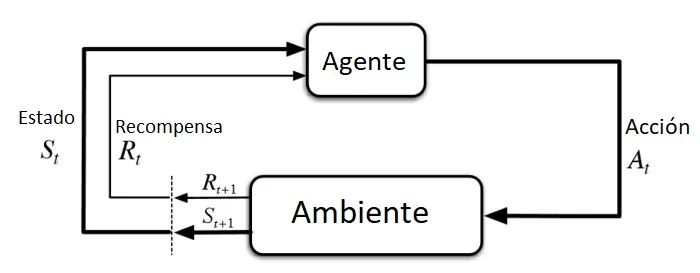
\includegraphics[width=0.9\linewidth]{imagenes_articulos/sp55_02} \end{center}
\figcaption{Diagrama del aprendizaje por refuerzo. Fuente: Reinforcement Learning: An Introduction.}

\end{minipage}
\end {flushleft}

La aplicación del aprendizaje por refuerzo en el mantenimiento de software ha mostrado resultados prometedores. La implementación de modelos de aprendizaje por refuerzo ha permitido reducir significativamente el tiempo necesario para identificar y corregir errores en sistemas complejos. En general, las técnicas basadas en aprendizaje por refuerzo han
reducido los tiempos de inactividad, mejorando la disponibilidad y la confiabilidad del software.

\hypertarget{conclusiones-9}{%
\section{Conclusiones}\label{conclusiones-9}}

El mantenimiento de software es crucial no solo para corregir errores, sino para garantizar la estabilidad, seguridad y adaptación de las aplicaciones a un entorno tecnológico en constante evolución. Un software bien mantenido minimiza las interrupciones y las vulnerabilidades, asegurando su relevancia y funcionalidad a largo plazo.

La integración de la inteligencia artificial, especial-
mente a través del aprendizaje por refuerzo, ha revolucionado el mantenimiento de software. Al automatizar tareas complejas y permitir que los sistemas aprendan y se adapten de forma autónoma, se ha logrado optimizar procesos, reducir tiempos de inactividad y mejorar la eficiencia operativa del software.

\hypertarget{referencias-8}{%
\section{Referencias}\label{referencias-8}}

\begin{itemize}
\item
  {[}1{]} Amazon Web Services, Inc.~¿Qué es el aprendizaje por refuerzo?. Última modificación en 2024.
  \href{https://aws.amazon.com/es/what-is/reinforcement-learning/}{https://aws.amazon.com}
\item
  {[}2{]} Rantanen, Oula. Artificial Intelligence in Software Maintenance. Master's thesis, LUT University, 2021. \href{https://lutpub.lut.fi/handle/10024/163419}{https://lutpub.lut.fi}
\item
  {[}3{]} Spyro-Soft. What Is Software Maintenance and Why It Is Essential. Consultado el 18 de agosto de 2024. \href{https://spyro-soft.com/blog/managed-services/what-is-software-maintenance-and-why-it-is-essential}{https://spyro-soft.com}
\item
  {[}4{]} Sutton, Richard S., y Andrew G. Barto. Reinforcement Learning: An Introduction. 2ª ed.~Cambridge, MA: MIT Press, 2018.
\end{itemize}

\end {multicols}

\medskip

\HRule

\medskip
%%%%%% SECCION 4
\includepdf{images/seccion4.pdf}

\AddEverypageHook{%
\ifthenelse{\value{page}<50}%
{\ifthenelse{\isodd{\value{page}}}%
  	{\backgroundsetup{scale=1, color=white, opacity=1, angle=0, contents={
\includegraphics[width=\paperwidth,height=\paperheight]{latex/background_numberimpar.pdf}}}}%
  	{\backgroundsetup{scale=1, color=white, opacity=1, angle=0, contents={
\includegraphics[width=\paperwidth,height=\paperheight]{latex/background_numberpar.pdf}}}}%
}{}%
\BgMaterial}
%%%%%%%%%%%%%%%%%%%%%%%%%%%
\hypertarget{ricardo}{%
\chapter{Visión Analítica: Revelando el poder de los datos y el Big Data}\label{ricardo}}

\begin{center}
\includegraphics[width=1\linewidth]{autores/pareja00_ricardo} \end{center}

\begin {multicols}{2}

\textbf{\emph{YouTube:}} \url{https://youtu.be/GwVJMtHVYOE}

\hypertarget{entrevista-3}{%
\section{Entrevista}\label{entrevista-3}}

\textbf{¿Quién es Ricardo Girón? ¿Cuál es su trayectoria profesional?}

Ricardo Girón es un san carlista apasionado por la docencia, con más de 25 años de experiencia en tecnología. Actualmente enseña en escuelas de posgrado, incluyendo la Universidad de San Carlos de Guatemala y escuelas de negocios. Es ingeniero en sistemas y cuenta con dos maestrías: una en proyectos y otra en finanzas. También ha iniciado estudios de doctorado en innovación tecnológica educativa y tiene certificación de Project Manager por el PMI. En su tiempo libre, disfruta del fútbol, toca la guitarra y juega billar.

\textbf{¿Cómo ha sido su participación en la industria tecnológica? ¿Qué experiencia ha acumulado en el área de Big Data?}

Ricardo Girón tiene más de 25 años de experiencia en tecnología, comenzando su carrera como progra-
mador a finales de los 90, trabajando con lenguajes como C++, Visual Basic y FoxBase. A lo largo de su trayectoria, ha evolucionado desde analista de sistemas hasta dirigir áreas de desarrollo de software, colaborando con plataformas importantes como Microsoft y Oracle. Destaca su trabajo en Formulario Estándar, una de las principales fábricas de formularios en Centroamérica, donde amplió su conocimiento en software y administración de infraestructura tecnológica.

En los últimos 10 a 15 años, ha trabajado en empresas de consultoría, incluyendo más de una década en SAP, donde ha gestionado equipos de proyectos. Esta experiencia le ha permitido entender diversos sectores e industrias, desde fábricas hasta bancos y retail, enriqueciendo su trayectoria profesional.

\bigskip
\bigskip
\bigskip
\bigskip
\bigskip
\bigskip

\textbf{¿Cómo ha evolucionado el análisis de los datos hasta llegar a la gran ola de transformación e innovación digital y Big Data, a la cual nos enfrentamos hoy día?}

La relación entre Big Data y el análisis de datos ha cambiado drásticamente, pasando de centrarse en pequeños volúmenes de datos estructurados a manejar grandes cantidades de información de diversas fuentes y formatos. Antes, las herramientas de análisis eran limitadas en capacidad de almacena-
miento y procesamiento. Hoy, gracias a tecnologías como Hadoop y Spark, es posible procesar enormes volúmenes de datos de manera ágil y escalable.

\textbf{¿Cuáles son las principales técnicas y métodos que se pueden utilizar para el procesamiento y análisis de estos grandes volúmenes de datos? ¿Qué herramientas nos pueden apoyar en el procesamiento de datos?}

Entre las técnicas comunes para procesar grandes volúmenes de datos se destacan los Data Warehouses, que consolidan la información de diferentes áreas de una organización, como ventas y finanzas. A medida que las empresas crecen, aumenta la necesidad de resumir y homologar datos, utilizando herramientas ETL (Extract, Transform, Load) para cargarlos en estos almacenes.

Además, herramientas como R y Python permiten a los usuarios finales realizar análisis estadísticos y procesar grandes cantidades de información, superando las limitaciones de Excel. Plataformas como Microsoft Power BI, Tableau, QlikView y MicroStrategy son accesibles para empresas de todos los tamaños, desde emprendedores hasta grandes corporaciones.

\textbf{¿De qué manera las técnicas de análisis de Big Data influyen en la toma de decisiones estratégicas empresariales? ¿Qué tipos de decisiones se ven más beneficiadas?}

Las técnicas de análisis de Big Data impactan profundamente en la toma de decisiones estratégicas de empresas y organizaciones al transformar su enfoque para resolver problemas y identificar oportunidades.

En primer lugar, el análisis predictivo mejora la precisión y reduce la incertidumbre, permitiendo pronosticar variables clave como ventas y costos.

Además, Big Data mejora la experiencia del cliente al fortalecer la segmentación y captar mejor su atención. También optimiza los procesos operativos, ayudando a las empresas a utilizar sus recursos de manera más eficiente. Otro beneficio es la detección de riesgos y fraudes, especialmente en sectores como el financiero, donde el monitoreo de transacciones es crucial.

Finalmente, Big Data impulsa la innovación y el desarrollo de nuevos productos al permitir a las empresas anticiparse a las expectativas de sus clientes. Un ejemplo de esto es cómo Apple utiliza el conocimiento generado a partir de sus usuarios para mejorar y lanzar nuevos productos.

\textbf{¿Cómo influyen las ``V'' del Big Data (Velocidad, Variedad, Volumen, Valor, Variabilidad) en la capacidad de las empresas de la Industria 4.0 para aprovechar los datos generados?}

Para que un conjunto de datos sea considerado Big Data, debe cumplir con las \textbf{``V''} del Big Data. La primera es \textbf{\emph{velocidad}}, que indica que los datos se generan rápidamente. La segunda es \textbf{\emph{variedad}}, que abarca tanto datos estructurados (números, textos) como no estructurados (fotos, redes sociales, videos, audios). La tercera es \textbf{\emph{volumen}}, que se refiere a la gran capacidad de almacenamiento de datos, que puede llegar a magnitudes como los yotabytes y generar millones de registros por minuto.

La cuarta \textbf{``V''} es \textbf{\emph{valor}}, lo que implica que los datos deben ser relevantes y útiles para la empresa. Por último, Big Data es \textbf{\emph{variable}}, ya que la producción de datos puede fluctuar según el tiempo y contexto, lo que afecta su gestión y análisis.

\textbf{¿Cómo se compara la generación de datos con la actividad que ocurre en Internet en un solo minuto?}

En 2023, se generaron 241.2 millones de correos electrónicos enviados y 41.6 millones de mensajes de WhatsApp por minuto. Además, hay 6.3 millones de búsquedas en Google cada minuto y 452,000 horas de video visualizadas en Netflix en el mismo período. Estas cifras reflejan lo que constituye Big Data, que cumple con las \textbf{``V''} del Big Data.

En Guatemala y Centroamérica, ejemplos de Big Data encontramos a las empresas de telecomunicacio-
nes, que pueden registrar millones de llamadas y mensajes diariamente, así como a los bancos que gestionan múltiples transacciones con tarjetas de crédito en sus agencias y puntos de venta. Todo esto representa un claro uso de Big Data en la región.

\begin {flushleft}
\noindent\begin{minipage}[c]{\columnwidth}

\begin{center}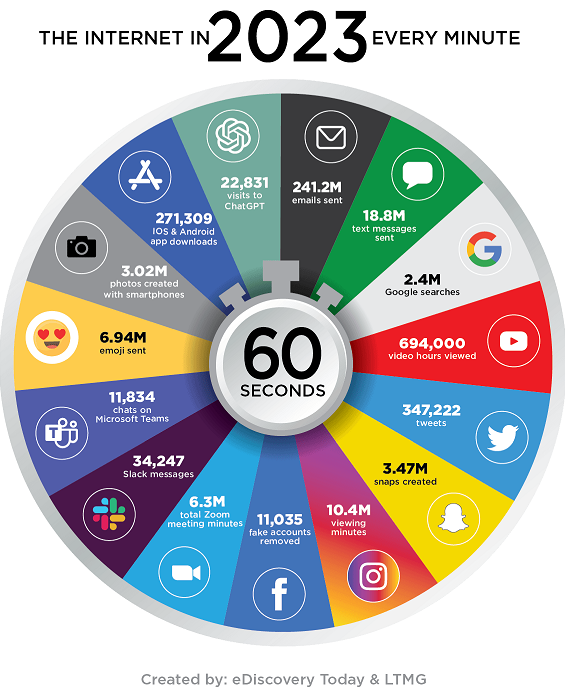
\includegraphics[width=1\linewidth]{imagenes_articulos/spricardo_01} \end{center}
\figcaption{. Fuente: }

\end{minipage}
\end {flushleft}

\textbf{¿Cómo afectan los roles de arquitecto de datos y científico de datos la capacidad de una organización para progresar en las etapas del análisis de datos? ¿Qué habilidades son esenciales para optimizar la toma de decisiones en cada tipo de análisis?}

Con el desarrollo del análisis de datos, han surgido nuevos roles como el analista de datos, el arquitecto de datos y el científico de datos. El analista de datos se especializa en identificar patrones y procesar información en un área específica de la empresa. El arquitecto de datos diseña la estructura de un Data Warehouse, mapeando las fuentes de información necesarias. Por su parte, el científico de datos se enfoca en desarrollar modelos predictivos y simulaciones con grandes volúmenes de datos, mejorando la toma de decisiones a través de análisis descriptivos, predictivos y perceptivos.

Las empresas adoptan estas prácticas progresiva-
mente, siguiendo un modelo de madurez. Por ejemplo, una cafetería puede comenzar registrando operaciones en Excel y, con el tiempo, evolucionar hacia el uso de modelos predictivos que optimizan pronósticos y reducen riesgos.

\textbf{¿Cómo impactan las técnicas avanzadas de procesamiento y análisis de grandes volúmenes de datos en el diseño y la arquitectura de un sistema de inteligencia de negocios? ¿Cuáles son los componentes clave para garantizar eficiencia y escalabilidad en un entorno de Big Data?}

Las técnicas de análisis de grandes volúmenes de datos requieren una arquitectura de inteligencia de negocios que integre Big Data. Este modelo incluye cuatro componentes clave:

\textbf{\emph{1. Fuentes de información:}} cualquier sistema o base de datos.

\textbf{\emph{2. Proceso de transformación (ETL):}} que extrae, transforma y carga la información.

\textbf{\emph{3. Almacenamiento:}} abarcando Data Warehouses, Data Lakes y Data Marts.

\textbf{\emph{4. Capa de presentación:}} donde se utilizan herramientas de análisis como Power BI y Tableau.

Esta arquitectura permite a los usuarios acceder a datos confiables y en tiempo real para la toma de decisiones. Para elegir las mejores soluciones tecnológicas, se pueden usar herramientas como el cuadrante de Gartner, que clasifica proveedores en diversas áreas.

El Big Data mejora la toma de decisiones y la experiencia del cliente, como se observa en plataformas de comercio electrónico que personalizan ofertas. También optimiza las cadenas de suministro al reducir costos y tiempos. Sin embargo, la implementación y mantenimiento de estas platafor-
mas presentan desafíos tanto en el sector privado como en el público.

\textbf{¿De qué manera las herramientas y plataformas recomendadas por Gartner Group influyen en la implementación y gestión de arquitecturas de Data Warehouse y Data Lake? ¿Cuáles son las principales consideraciones para integrar estas tecnologías en un entorno de análisis de datos?}

Gartner es una firma internacional que anualmente califica y clasifica a los mejores proveedores de tecnología en diversas áreas, como sistemas contables financieros, Data Warehouses y soluciones de inteligencia de negocios. Utiliza un cuadrante que ayuda a las empresas a identificar qué herramientas de análisis de datos son más adecuadas para sus necesidades.

Dado el gran número de opciones disponibles, Gartner se convierte en un referente útil para evaluar soluciones y tomar decisiones informadas. Su evaluación permite a las empresas implementar arquitecturas de Data Warehouse, Data Lake y soluciones en la nube, asegurándoles que están eligiendo opciones estables, probadas y con un futuro innovador.

\textbf{¿Cómo ha transformado el uso de Big Data las estrategias y operaciones en sectores clave como marketing, servicio al cliente, comercio y el sector público? ¿Cuáles son los beneficios y desafíos específicos en cada uno de estos ámbitos?}

La mejora en la toma de decisiones y la experiencia del cliente se refleja en cómo las plataformas de comercio electrónico, como Amazon, personalizan ofertas y recomendaciones, aumentando la satisfacción y lealtad del cliente. Estas empresas utilizan Big Data e inteligencia artificial para entender el comportamiento y las necesidades de sus clientes, lo que resulta en una mejor atención.

A nivel operativo, Big Data optimiza las cadenas de suministro, mejorando rutas de distribución, reduciendo tiempos de espera y costos, y aumentando la trazabilidad de productos. En cuanto a la innovación, ayuda a identificar necesidades no satisfechas, permitiendo la creación de soluciones más efectivas.

Sin embargo, tanto el sector privado como el público enfrentan desafíos. En el sector privado, las empresas deben evaluar y mantener soluciones adecuadas y contar con personal capacitado. En el sector público, como en proyectos de la Municipalidad de Guatemala y el Ministerio de Finanzas, se busca procesar información para mejorar servicios, aunque la selección e implementación de plataformas de análisis de datos sigue siendo un reto.

\textbf{¿Qué retos trae a los estudiantes y profesionales esta revolución tecnológica 4.0, respecto al análisis de datos y Big Data? ¿Cómo visualiza el futuro del análisis de datos a corto y largo plazo?}

La recomendación para profesionales y estudiantes es mantenerse actualizados en un mundo en constante cambio, combinando teoría con práctica en el análisis de datos. La práctica es fundamental, ya que instalar y probar herramientas de análisis puede ser muy beneficioso. Este desafío es relevante para todos, dado que la Revolución Industrial 4.0 y el análisis de datos se aplican en diversas áreas de negocio y en muchos aspectos de la vida. Es crucial que cada interesado busque su propio enfoque y se sumerja en estos temas para aprovechar las oportunidades que ofrecen.

\bigskip
\bigskip
\bigskip

\textbf{¿Qué mensaje les daría a quienes desean adentrarse en el mundo del Big Data y el análisis de datos?}

La famosa frase de Francis Bacon, \emph{``El conocimiento es poder''}, ha evolucionado a \emph{``Quien tiene la información, tiene el poder''}. Esto refleja la realidad actual, donde la capacidad de obtener, procesar y analizar datos impacta directamente en la toma de decisiones y el futuro profesional. Las decisiones basadas en información conducen a mejores resultados y mayor especialización.

En el futuro, surgirán oportunidades en áreas donde la inteligencia artificial aún no puede intervenir, aunque su velocidad para procesar datos supera a la humana. Por lo tanto, es crucial combinar la inteligencia artificial con el análisis humano para tomar decisiones informadas que beneficien a las empresas y los negocios. Esa es la clave para un futuro exitoso.

\end {multicols}

\medskip

\HRule

\medskip

\hypertarget{pareja16}{%
\chapter{Transformando digitalmente nuestras aduanas, un paso hacia el futuro}\label{pareja16}}

\begin{center}\includegraphics[width=1\linewidth]{autores/pareja16_01} \end{center}

\begin {multicols}{2}

\textbf{\emph{Palabras clave:}} Aduanas, Big Data, Modernización, Transformación digital, Innovación tecnológica.

\hypertarget{introducciuxf3n-10}{%
\section{Introducción}\label{introducciuxf3n-10}}

La transformación digital es un tema el cual año con año se ha visto más necesario, especialmente en tiempos recientes donde varias actividades se vieron limitadas, fue en este momento que esto se convirtió en un reto e implicó la toma de nuevas medidas, gracias a ello se impulsaron distintos proyectos de digitalización en combinación de múltiples tecnologías.

Entre las áreas que pusieron manos a la obra y tomaron acciones tenemos las aduanas las cuales hoy en día han demostrado múltiples beneficios, desde el más simple que es el ahorro del papel necesario para la realización de las distintas gestiones, hasta otros más avanzados y complejos como proyectos de automatización y modernización.

\hypertarget{artuxedculo-10}{%
\section{Artículo}\label{artuxedculo-10}}

Las aduanas son parte fundamental de las operaciones de una nación ya que estas son esenciales al cumplir con actividades como asegurar la seguridad del país, aportar a la economía, regular el comercio internacional, gestionar el proceso de libre plática, el cual se refiere al procedimiento de autorización necesario según instituciones gubernamentales para que una nave, buque u otro medio de transporte pueda realizar las acciones de embarque y
desembarque correspondientes, entre otras características adiciona-
les que en conjunto ayudan a mejorar el bienestar general de la nación.

Debido a su gran importancia para el país y al papel que representa en las distintas industrias que hacen uso de estas, se han buscado soluciones para poder acelerar los procesos, manteniendo y en lo posible mejorando los resultados, siendo en este punto donde entran en juego aspectos como la digitalización, Big Data, automatización y demás tecnologías. Encaminandonos un poco más a proyectos con un objetivo claro y específico encontramos múltiples proyectos de modernización, de uso de tecnologías de datos, y de avance de la infraestructura tecnológica, como lo son los descritos a continuación:

\textbf{MIAD (Modelo de Información Aduanera Digitali-
zada)}

Este proyecto, iniciado en 2019, busca modernizar y digitalizar la gestión aduanera para mejorar la eficiencia y reducir el fraude mediante análisis predictivo que detecta patrones inusuales en las transacciones aduaneras, identificando fraudes y evasión fiscal. Un pilar clave del proyecto es eliminar el uso de papel mediante firmas electrónicas para gestionar de manera segura y controlada los cambios de estado en los flujos del proceso.

\textbf{VUMAR (Ventanilla Única Marítima)}

Proyecto conformado por las 5AG (Ministerio de la Defensa Nacional; SAT; Ministerio de Agricultura, Ganadería y Alimentación; Ministerio de Salud Pública y Asistencia Social; Instituto Guatemalteco de Migración), tiene por objetivo principal centralizar y simplificar los procesos aduaneros marítimos tales como lo son la Libre Plática mediante una plataforma digital integrada, que permite la gestión eficiente y segura de las operaciones de comercio
marítimo. El sistema busca modernizar y digitalizar la gestión aduanera marítima para mejorar la eficiencia y reducir riesgos siguiendo el ejemplo de MIAD.

Entre otros proyectos y tecnologías podemos mencionar los siguientes:

\begin {flushleft}
\noindent\begin{minipage}[c]{\columnwidth}

\includegraphics[width=1\linewidth]{imagenes_articulos/sp16_01}
\tabcaption{Proyectos y tecnologías usados en la transformación digital de aduanas. Fuente: Elaboración propia con datos obtenidos de portal SAT.}

\end{minipage}
\end {flushleft}

\bigskip
\bigskip
\bigskip
\bigskip

Como reflejo de las mejoras y avances en las implementaciones tecnológicas en las aduanas se puede visualizar un incremento significativo en lo que es la carga tributaria que se mide como el porcentaje del Producto Interno Bruto (PIB) que representa la recaudación de impuestos del gobierno central, posiblemente debido a la reactivación económica y a las medidas de mejora en la recaudación tributaria.

\bigskip
\bigskip

\begin {flushleft}
\noindent\begin{minipage}[c]{\columnwidth}

\begin{center}\includegraphics[width=1\linewidth]{imagenes_articulos/sp16_02} \end{center}
\figcaption{Comportamiento de la recaudación anual como porcentaje del PIB. Fuente: Portal SAT - https://goo.su/K8Xve}

\end{minipage}
\end {flushleft}

\bigskip
\bigskip
\bigskip
\bigskip
\bigskip
\bigskip
\bigskip
\bigskip

\hypertarget{conclusiones-10}{%
\section{Conclusiones}\label{conclusiones-10}}

En la búsqueda de alcanzar el objetivo de transformación digital de las aduanas se ha logrado la implementación de diversos proyectos en conjunto con la integración de nuevas tecnologías, las cuales han brindado una gran cantidad de mejoras y beneficios, tanto a nivel de aduanas, mejorando las condiciones y calidad de servicio, ayudando en las tareas administrativas, reduciendo la carga de los empleados de igual manera que el tiempo empleado para cada caso, así como a una escala y alcance mayor representando un impacto a nivel de nación, como lo es para el sector económico permitiendo por ejemplo mejorar la precisión y eficiencia en la recaudación de tributos por parte de la Superintendencia de Administración Tributaria (SAT) lo que representa un impacto positivo en la mejora del bienestar general de la nación.

\hypertarget{referencias-9}{%
\section{Referencias}\label{referencias-9}}

\begin{itemize}
\item
  {[}1{]} Global Alliance for Trade Facilitation. ``Guate-
  mala launches transformative Maritime Single Window (VUMAR).''
  3 de mayo de 2024.Accedido el 2 de agosto de 2024. \href{https://www.tradefacilitation.org/article/guatemala-launches-transformative-maritime-single-window-vumar/}{https://www.tradefacilita-
  tion.org}
\item
  {[}2{]} SEAL: Servicios Especializados de Aduana y Logística, S. A. ``Digitalización de las aduanas en Latinoamérica.''
  21 de diciembre de 2021. \href{https://www.seal.com.gt/digitalizacion-de-las-aduanas-en-latinoamerica/}{https://www.seal.com.gt}
\item
  {[}3{]} Superintendencia de Administración Tributaria (SAT). ``Estadísticas Tributarias.'' Accedido el 2 de agosto de 2024. \href{https://portal.sat.gob.gt/portal/estadisticas-tributarias-sat/\#1506903647232-dff79679-679a}{https://portal.sat.gob.gt}
\end{itemize}

\end {multicols}

\medskip

\HRule

\medskip

\hypertarget{pareja57}{%
\chapter{Hacia dónde se dirige Latinoamérica: El impacto del Big Data y análisis de datos}\label{pareja57}}

\begin{center}\includegraphics[width=1\linewidth]{autores/pareja57_01} \end{center}

\begin {multicols}{2}

\textbf{\emph{Palabras clave:}} Big Data, Latinoamérica, Análisis de datos, Internet de las cosas, Inteligencia artificial.

\hypertarget{introducciuxf3n-11}{%
\section{Introducción}\label{introducciuxf3n-11}}

El análisis de datos ha evolucionado de manera exponencial, y su impacto es cada vez más palpable en diversos sectores como la industria, la agroindustria, la economía e incluso la medicina. Todos estos campos, entre otros, tienen la capacidad de extraer información valiosa de grandes volúmenes de datos y están revolucionando la forma en que operan las industrias.

En Latinoamérica, esta tendencia se está consoli-
dando como un motor crucial para la innovación y el crecimiento económico. Sin embargo, la región enfrenta desafíos y oportunidades únicas que deben ser abordados para evitar que el progreso se vea obstaculizado.

\hypertarget{artuxedculo-11}{%
\section{Artículo}\label{artuxedculo-11}}

En los últimos años, Latinoamérica ha visto un aumento en la generación de datos, impulsado por la digitalización de procesos en sectores clave como la salud, especialmente tras la pandemia del COVID-19, que generó un gran volumen de datos, el transporte y la educación.

Según un informe de IDC, se espera que el mercado de TI en Latinoamérica crezca un 11.1\% en 2024, alcanzando 81.2 mil millones de dólares. Este crecimiento refleja la creciente inversión en infraestructura tecnológica y la adopción de soluciones analíticas avanzadas por parte de las empresas de la región.

A medida que el análisis de datos evoluciona, Brasil y México se destacan como los principales líderes en la adopción de Big Data, impulsando algunas de las tendencias más emergentes en la región, como la inteligencia artificial, la analítica predictiva y la integración del Internet de las Cosas (IoT).

En Brasil, NeuralMind utiliza técnicas avanzadas de IA para detectar fraudes en el sistema eléctrico. Esta iniciativa comenzó en 2019 y utiliza IoT para monitorear el consumo de energía en tiempo real y detectar discrepancias que podría indicar fraudes. Es uno de los pocos proyectos a nivel mundial que integra datos de consumo y generación de energía.

Por otra parte, México ha avanzado significativa-
mente en la adopción del IoT para optimizar la eficiencia de la producción y el mantenimiento predictivo. En 2023, durante el evento Automotive Logistics and Supply Chain Mexico, Volkswagen detalló cómo están aprovechando herramientas digitales para gestionar grandes volúmenes de datos de su
cadena de suministro, reduciendo riesgos y mejorando la rentabilidad.

Mientras tanto, en Argentina las instituciones financieras han comenzado a utilizar modelos predictivos para enfrentar desafíos económicos significativos, como la inflación y la volatilidad del mercado cambiario. Un ejemplo reciente es el uso de modelos Random Forest para predecir la inflación mensual, los cuales analizan datos históricos para detectar
patrones y cuya precisión es comparable a métodos econométricos tradicionales.

\textbf{Desafíos y oportunidades en la región}

A pesar de las numerosas oportunidades que presenta la adopción de Big Data en Latinoamérica, la región se enfrenta a una serie de desafíos significativos que podrían ralentizar su progreso. Estos desafíos incluyen limitaciones en la infraestructura tecnológica, una escasez de talento especializado en análisis de datos, y la necesidad de marcos regulatorios robustos que garanticen la privacidad y seguridad de los datos.

\emph{\textbf{Infraestructura tecnológica}}

Aunque se han realizado avances, la infraestructura tecnológica en muchos países de la región sigue siendo insuficiente. La conectividad a Internet y la capacidad de almacenamiento de datos son áreas que requieren mejoras sustanciales. Las áreas rurales en su mayoría siguen rezagadas en conectividad y acceso a servicios. La falta de adopción de la red 5G conlleva a una disparidad significativa en velocidad y calidad de acceso.

\begin {flushleft}
\noindent\begin{minipage}[c]{\columnwidth}

\begin{center}\includegraphics[width=1\linewidth]{imagenes_articulos/sp57_01} \end{center}
\figcaption{Adopción de red 5G en Latinoamérica. Fuente: https://goo.su/xz6dBP}

\end{minipage}
\end {flushleft}

\emph{\textbf{El arte es cada vez más accesible para más personas}}

Escasez de talento especializado. Existe una brecha en la disponibilidad de profesionales capacitados en análisis de datos.Las universidades y centros de formación están comenzando a desarrollar programas específicos para cerrar esta brecha, pero aún queda camino por recorrer.

\emph{\textbf{Regulación y privacidad de datos}}

La regulación en torno a la privacidad de los datos es otro desafío crítico. Países como México y Colombia han comenzado a implementar leyes de protección de datos, pero la consistencia y aplicación de estas regulaciones varía ampliamente en la región.

\hypertarget{conclusiones-11}{%
\section{Conclusiones}\label{conclusiones-11}}

El análisis de datos en Latinoamérica está en una etapa crucial de desarrollo, marcada por un dinamismo que promete transformar diversos sectores económicos y sociales. Aunque la región enfrenta desafíos significativos en términos de infraestructura, como la falta de conectividad en áreas rurales, y regulación, especialmente en la protección de datos, las oportunidades para innovar y crecer son inmensas. El aumento en la adopción de tecnologías avanzadas, como la inteligencia artificial (IA) y el Internet de las Cosas (IoT), están abriendo nuevas vías para el análisis de grandes volúmenes de datos en tiempo real. Es esencial que los países de la región adopten una visión proactiva y colaborativa, invirtiendo en el desarrollo de infraestructuras robustas y en la capacitación del talento local, para superar las barreras existentes y aprovechar al máximo el potencial del Big Data.

\hypertarget{referencias-10}{%
\section{Referencias}\label{referencias-10}}

\begin{itemize}
\item
  {[}1{]} Dhamnekar, Sushant, Andrea Ketzer, y Chandana Keswarkar. ``Recap of AWS re:Invent 2023 for the Automotive Industry.'' AWS Blog. \href{https://aws.amazon.com/es/blogs/industries/recap-of-aws-reinvent-2023-for-the-automotive-and-manufacturing-industry/}{https://aws.amazon.com}
\item
  {[}2{]} Forte, Federico D. ``Pronóstico de Inflación de Corto Plazo en Argentina con Modelos Random Forest.'' BBVA
  Research. \href{https://www.bbvaresearch.com/publicaciones/pronostico-de-inflacion-de-corto-plazo-en-argentina-con-modelos-random-forest/}{https://www.bbvarese-
  arch.com}
\item
  {[}3{]} International Data Corporation (IDC). ``A partir de 2024, empresas de TI de Latinoamérica tendrán un crecimiento
  más estable que las de EEUU, según IDC.'' IDC. \href{https://www.idc.com/getdoc.jsp?containerId=prLA51751624}{https://www.idc.com}
\item
  {[}4{]} Murcia, Paula. ``Protección de Datos: Este es el Panorama Sobre Regulación en Latinoamérica'' Valora Analitik. \href{https://www.valoraanalitik.com/proteccion-de-datos-este-es-el-panorama-sobre-regulacion-en-latinoamerica/}{https://www.valoraanalitik.com}
\item
  {[}5{]} NeuralMind. ``Projeto aplica técnicas avançadas de Inteligência Artificial para detectar fraudes no setor elétrico.'' NeuralMind Blog. \href{https://neuralmind.ai/blog/projeto-aplica-tecnicas-avancadas-de-inteligencia-artificial-para-detectar-fraudes-no-setor-eletrico/}{https://neural-
  mind.ai}
\end{itemize}

\end {multicols}

\medskip

\HRule

\medskip

\hypertarget{pareja19}{%
\chapter{Big Data en la transformación del sector financiero}\label{pareja19}}

\begin{center}\includegraphics[width=1\linewidth]{autores/pareja19_01} \end{center}

\begin {multicols}{2}

\textbf{\emph{Palabras Clave:}} Big Data, Finanzas, Análisis, Herramientas, Transacciones, Predicción.

\hypertarget{introducciuxf3n-12}{%
\section{Introducción}\label{introducciuxf3n-12}}

Big Data es el análisis de enormes cantidades de datos variados y complejos para descubrir patrones y tendencias útiles, ayudando a tomar decisiones más informadas. En el sector financiero, la adopción de esta tecnología ha traído consigo numerosas ventajas que han llevado el manejo y análisis de inmensos volúmenes de datos al siguiente nivel.

En un mercado que genera abundante información sobre clientes, productos financieros, transacciones, entre otros, Big Data ha cambiado las reglas del juego. Las empresas buscan herramientas y modelos que permitan predecir con mayor precisión el comportamiento de inversiones, oportunidades de venta y la satisfacción del cliente, lo que les ayuda a sobrevivir y adaptarse en un entorno altamente competitivo.

\hypertarget{artuxedculo-12}{%
\section{Artículo}\label{artuxedculo-12}}

Para abordar la predicción y el análisis de mercados financieros utilizando Big Data, es esencial establecer una ruta a seguir, el primer punto de partida es seleccionar adecuadamente las fuentes de datos. A diferencia de los datos tradicionales, que suelen ser estructurados y provienen de fuentes bien definidas como bases de datos transaccionales y registros históricos, las fuentes de Big Data son mucho más variadas y voluminosas. Estas incluyen datos no estructurados, por ejemplo, de redes sociales, noticias, blogs, transacciones en línea y datos generados por sensores, entre otros.

Al seleccionar las fuentes de Big Data, debemos enfocarnos en aquellas que proporcionan información relevante y actualizada, además, es fundamental implementar tecnologías avanzadas para la recolec-
ción, almacenamiento y procesamiento de estos datos masivos, permitiendo así su análisis efectivo. Este proceso no solo enriquece la calidad de las predicciones, sino que también complementa los datos tradicionales, ofreciendo una perspectiva integral y robusta para la toma de decisiones financieras.

Teniendo establecidas las fuentes de datos, procedemos a definir las herramientas de Big Data, una de ellas es Apache Kafka, una plataforma distribuida de transmisión de datos que está transfor-
mando la forma en cómo se procesan los datos financieros en la nube, su capacidad para manejar volúmenes masivos de datos en tiempo real de forma rápida, segura y con alto rendimiento la está convirtiendo en una de las principales opciones por miles de instituciones financieras que buscan aumentar sus capacidades de procesamiento de datos.

El framework Hadoop también se ha convertido en una de las herramientas preferidas de Big Data en el mercado financiero, especialmente para gestionar algunos de los retos más comunes para cualquier entidad de este tipo como lo es el fraude, los delitos financieros y la corrupción de datos.

\begin {flushleft}
\noindent\begin{minipage}[c]{\columnwidth}

\begin{center}\includegraphics[width=1\linewidth]{imagenes_articulos/sp19_01} \end{center}
\figcaption{Tamaño y alcance del mercado mundial de análisis de big data en banca. Fuente: https://goo.su/MZiwugA}

\end{minipage}
\end {flushleft}

El Big Data es un término común, pero a veces difícil de concretar. Sin embargo, su uso por grandes empresas demuestra claramente sus beneficios en los mercados financieros. A continuación, un caso de éxito que ilustra su impacto.

La empresa estadounidense American Express (AmEx) es un claro ejemplo de los beneficios del uso de Big Data en el sector financiero. Al analizar enormes cantidades de datos provenientes de propietarios de tarjetas de crédito, logran detectar y limitar las transacciones fraudulentas, al mismo tiempo que proporcionan un proceso de compra eficiente. Esto es posible gracias a una herramienta creada por la propia empresa, llamada Enhanced Authorization, la cual permite obtener información sobre quién realiza cada transacción, para posteriormente compararla con la almacenada en su base de datos y prevenir el fraude.

\hypertarget{conclusiones-12}{%
\section{Conclusiones}\label{conclusiones-12}}

Es de suma importancia seleccionar adecuadamente las fuentes de datos en el contexto de Big Data, especialmente al incluir datos no estructurados de redes sociales, noticias, blogs y transacciones, lo que enriquece el análisis pero complica su recolección y procesamiento.

El uso de herramientas avanzadas de Big Data, como Apache Kafka y Hadoop, es fundamental para mejorar la toma de decisiones financieras, al manejar grandes volúmenes de datos en tiempo real y resolver desafíos como la detección de fraudes y la gestión de riesgos.

Los casos de éxito en el uso de Big Data en el sector financiero, como el de American Express, muestran su valor práctico al mejorar la eficiencia operativa y ofrecer ventajas competitivas, optimizando la detección de fraudes y la experiencia del cliente.

\hypertarget{referencias-11}{%
\section{Referencias}\label{referencias-11}}

\begin{itemize}
\item
  {[}1{]} Abraham, Facundo, Sergio L. Schmukler y José Tessada. ``Using Big Data to Expand Financial Services: Benefits and Risks''. Research \& Policy Briefs - World Bank Group, n.º 26 (noviembre de 2019).
  \href{https://documents1.worldbank.org/curated/en/505891573224492672/pdf/Using-Big-Data-to-Expand-Financial-Services-Benefits-and-Risks.pdf}{https://documents1.worldbank.org}
\item
  {[}2{]} Domínguez, Sandra. ``Impacto del Big Data en la gestión de riesgos en el sector financiero''. OpenWebinars (septiembre de 2023). Consultado el 31 de julio de 2024. \href{https://openwebinars.net/blog/impacto-del-big-data-en-la-gestion-de-riesgos-en-el-sector-financiero}{https://openwebinars.net}
\item
  {[}3{]} ``Kafka for Cloud-Based Financial Data Processing: A Secure and Scalable Solution Alibaba Cloud''. Alibaba Cloud: Reliable Secure Cloud Solutions to Empower Your Global Business. Consultado el 2 de agosto de 2024.
  \href{https://www.alibabacloud.com/tech-news/a/kafka/gtv2q09gbd-kafka-for-cloud-based-financial-data-processing-a-secure-and-scalable-solution}{https://www.alibabacloud.com}
\item
  {[}4{]} Dutta, Subhasish. ``Big Data in Finance: Benefits, Use Cases, and Examples''. Expert GenAI Solutions \& LLM Training \textbar{} Turing. Consultado el 2 de agosto de 2024. \href{https://www.turing.com/resources/big-data-in-finance\#1.-predictive-analysis}{https://www.turing.com}
\end{itemize}

\end {multicols}

\medskip

\HRule

\medskip

\hypertarget{pareja40}{%
\chapter{Impacto del Big Data en la salud y la agricultura}\label{pareja40}}

\begin{center}\includegraphics[width=1\linewidth]{autores/pareja40_01} \end{center}

\begin {multicols}{2}

\textbf{\emph{Palabras clave:}} Big data, Salud, Internet de las cosas (IoT), Análisis de datos.

\hypertarget{introducciuxf3n-13}{%
\section{Introducción}\label{introducciuxf3n-13}}

El Big Data ha revolucionado numerosos campos, destacando especialmente en la salud y la agricultura. En el sector sanitario, el análisis de grandes volúmenes de datos permite fusionar información genética, clínica y conductual, favoreciendo tratamientos más personalizados y eficaces. Este enfoque no solo mejora la atención al paciente, sino que también promueve estrategias preventivas más efectivas, transformando fundamentalmente la práctica médica moderna.

En el ámbito agrícola, el Big Data está redefiniendo la gestión de recursos y la toma de decisiones. Al integrar datos de sensores IoT, información climática y análisis predictivos, los agricultores pueden optimizar la selección de cultivos, mejorar el rendimiento y adoptar prácticas más sostenibles.

\hypertarget{artuxedculo-13}{%
\section{Artículo}\label{artuxedculo-13}}

\textbf{Impacto del Big Data en la salud}

El Big Data ha transformado significativamente el sector de la salud, revolucionando tanto el tratamiento como la gestión de datos médicos. Esto ha llevado al desarrollo de modelos predictivos más eficientes que los métodos tradicionales, mejorando la prevención, el diagnóstico y el tratamiento de enfermedades.

Un ejemplo concreto es el Sistema de Monitoreo de Salud Inteligente Basado en Big Data, que integra aprendizaje profundo y ensemble learning para detectar patrones complejos en los datos de salud. Este sistema ofrece ventajas como:

\begin{itemize}
\item
  Alertas en tiempo real para intervenciones rápidas.
\item
  Identificación proactiva de riesgos de salud.
\item
  Mejora en la precisión y robustez de los modelos predictivos.
\end{itemize}

Sin embargo, también presenta desafíos como la privacidad y seguridad de los datos, la necesidad de grandes volúmenes de información y poder computacional, y la posibilidad de falsas alarmas o diagnósticos imprecisos.

El uso de análisis de datos es útil en el análisis masivo de registros médicos, lo cual permite generar modelos predictivos tanto para el diagnóstico como para la prevención de enfermedades pues mediante el análisis del lenguaje natural y la minería de datos es posible implementar prevención de riesgos y farmacovigilancia lo cual puede aportar a la practica terapeutica.

\begin {flushleft}
\noindent\begin{minipage}[c]{\columnwidth}

\begin{center}\includegraphics[width=1\linewidth]{imagenes_articulos/sp40_01} \end{center}
\figcaption{Arquitectura del sistema de monitoreo de salud basado en big data. Fuente: https://goo.su/LrFgA}

\end{minipage}
\end {flushleft}

Como se observa en la \emph{figura 22.1}, se muestra un flujo de trabajo para el sistema de monitoreo de salud, que está basado en sensores, los pacientes pueden ser monitoreados en tiempo real, lo cual provee un buen mapa de datos, los cuales mediante los algoritmos correspondientes, y usando tecnologías como machine learning se obtiene una predicción del desempeño terapéutico aplicado sobre un paciente concreto además de contribuir con la información predictiva para poder ser extrapolada a casos generales de uso.

\bigskip
\bigskip
\bigskip
\bigskip

\textbf{Aplicación de big data en agricultura}

En el sector agrícola, el Big Data está impulsando una revolución en la gestión de recursos naturales y la toma de decisiones. La implementación de algoritmos de agricultura inteligente, combinados con tecnología IoT, permite:

\begin{enumerate}
\def\labelenumi{\arabic{enumi}.}
\item
  Monitoreo detallado de factores ambientales (temperatura, humedad, presión atmosférica, contenido de humedad del suelo).
\item
  Recomendaciones precisas sobre la selección de cultivos basadas en condiciones específicas de la granja.
\item
  Análisis de correlación 3D para examinar técnicas de cultivo y cambios ambientales.
\end{enumerate}

Este enfoque mejora la eficiencia y sostenibilidad de la agricultura a gran escala, permitiendo decisiones más informadas sobre la selección de cultivos y técnicas agrícolas. A su vez puede tanto prevenir como impulsar, por lo cual el análisis de su productividad y sostenibilidad a largo plazo es crucial para analizar las implicaciones de esta tecnología en la sociedad.

Existen ya proyectos donde esto se ha llevado a cabo usando la tecnología IoT para vigilancia ambiental, seguido de un análisis de datos para determinar la mejor estrategia de cultivos según las condiciones espaciales y temporales, con esto se obtiene una mejor predicción del impacto económico y ambiental de un caso agrícola específico.

El proceso de normalización y limpieza de datos se realiza mediante promedios móviles y varianza para eliminar anomalías. Además, se emplea un análisis de correlación 3D para examinar las técnicas de cultivo y analizar los cambios ambientales provocados por el clima y la erosión del suelo.

El análisis de datos a mejorado la eficiencia y sostenibilidad de la agricultura a gran escala, dado que con un mayor manejo de las variables se pueden tomar mejores decisiones sobre la selección de cultivos y las técnicas agrícolas, basado en una gama más amplia de lecturas sobre las condiciones climáticas y ambientales, también produciendo una baja del riesgo climático asociado.

Con la implementación de la agricultura inteligente se puede mejorar el estudio de los entornos agrícolas y mejorar la toma de decisiones de diseño agrícola basado en los resultados experimentales, una habilidad crucial para la sostenibilidad dado el impacto del cambio climático a esta rama en concreto del conocimiento.

\hypertarget{conclusiones-13}{%
\section{Conclusiones}\label{conclusiones-13}}

El Big Data ha transformado radicalmente los sectores de la salud y la agricultura, catalizando innovaciones que mejoran la calidad de vida y la sostenibilidad. En la atención médica, ha permitido un monitoreo más preciso y una atención personalizada, mientras que en la agricultura ha optimizado la gestión de recursos y la toma de decisiones. No obstante, estos avances conllevan desafíos significativos en términos de privacidad, seguridad de datos e infraestructura.

A medida que estas tecnologías evolucionan, es crucial adaptar políticas y prácticas para maximizar sus beneficios. El impacto del Big Data va más allá de mejoras sectoriales, contribuyendo al bienestar general de la sociedad y sentando las bases para un desarrollo más sostenible e innovador. La discusión sobre cómo integrar éticamente estas tecnologías en nuestra vida cotidiana sigue abierta, planteando interrogantes sobre el futuro de la interacción entre la tecnología y la sociedad.

\hypertarget{referencias-12}{%
\section{Referencias}\label{referencias-12}}

\begin{itemize}
\item
  {[}1{]} Abidi, M. H., U. Umer, S. H. Mian, and A. Al-Ahmari. ``Big Data-Based Smart Health Monitoring System: Using Deep Ensemble Learning.'' IEEE Access 11 (2023): 114880 - 114883. \url{http://dx.doi.org/10.1109/ACCESS.2023.3325323}
\item
  {[}2{]} Andreu-Perez, Javier, Carmen Poon, Robert Merrifield, Stephen Wong, and Guang-Zhong Yang. ``Big Data for Health.'' IEEE Journal of Biomedical and Health Informatics 19, no. 4 (July 2015): 1193-1194. \url{http://dx.doi.org/10.1109/JBHI.2015.2450362}
\item
  {[}3{]} Tseng, Fan-Hsun, Hsin-Hung Cho, and Hsin-Te Wu. ``Applying Big Data for Intelligent Agriculture-Based Crop Selection Analysis.'' IEEE Access 7 (2019): 116965-116970. \url{http://dx.doi.org/10.1109/ACCESS.2019.2935564}
\end{itemize}

\end {multicols}

\medskip

\HRule

\medskip

\bibliography{book.bib,packages.bib}

%%%%\printindex



\includepdf{images/contraportada.pdf}


\end{document}
